\documentclass[aspectratio=169,11pt]{beamer}
\usetheme{metropolis}

\usepackage{amsmath,amssymb}
\usepackage{booktabs}
\usepackage{graphicx}
\usepackage{tikz}
\usepackage{algorithm2e}

\newcommand{\R}{\mathbb{R}}
\newcommand{\Gop}{\mathcal{G}}
% \tanh already defined by amsmath
\DeclareMathOperator{\rfft}{rfft}
\DeclareMathOperator{\irfft}{irfft}
\DeclareMathOperator{\relltwo}{rel\text{-}L^2}

\title{Learning the Dirichlet--Neumann Operator\\with Fourier Neural Operators}
\subtitle{Depth-conditioned surrogate modeling for nonlinear water waves}
\date{\today}
\author{Jonathan Ma}

\begin{document}

% ============================================================
\begin{frame}
\titlepage
\end{frame}

% ============================================================
\section{Problem Setup}

% ============================================================
\begin{frame}{The Dirichlet--Neumann Operator}

The free-surface Euler equations in Zakharov--Craig--Sulem form:
\begin{align}
  \eta_t &= \Gop(\eta;\,h)\,\xi, \label{eq:zt1}\\
  \xi_t &= -g\,\eta - \tfrac{1}{2}\xi_x^2
    + \frac{(\Gop(\eta;h)\xi + \eta_x\,\xi_x)^2}{2(1+\eta_x^2)}, \label{eq:zt2}
\end{align}
where $\eta(x,t)$ is surface elevation, $\xi(x,t)$ is surface velocity potential, $h$ is depth.

\pause
\textbf{$\Gop(\eta;\,h)\,\xi$} is the Dirichlet--Neumann operator: maps the surface potential $\xi$ to its (weighted) normal derivative at $z = \eta(x)$.

\pause
\textbf{Computational bottleneck:} Evaluating $\Gop$ requires solving Laplace's equation in the fluid domain at every time step. We compute it via the Craig--Sulem series:
\[
  \Gop(\eta;h)\,\xi = \sum_{m=0}^{M} G_m(\eta)\,\xi,
\]
truncated at order $M = 6$, with $8\times$-padded FFTs to avoid aliasing.
\end{frame}

% ============================================================
\begin{frame}{Goal}

\textbf{Replace} the expensive $\Gop(\eta;\,h)\,\xi$ evaluation with a neural surrogate:
\[
  \Gop(\eta;\,h)\,\xi \approx \hat{\Gop}_\theta(\eta,\,\xi;\, h).
\]

\pause
Requirements:
\begin{itemize}
  \item Accurate across wave regimes: solitons, Stokes waves, random sea states
  \item Generalize across depths: shallow water ($h = 1$) through deep water ($h = 1000$)
  \item Stable when plugged into a time integrator for long rollouts ($T \gg 100$)
\end{itemize}

\pause
Approach:
\begin{enumerate}
  \item Generate training data via high-fidelity numerical solvers
  \item Train a depth-conditioned FNO on $(\eta, \xi, h) \mapsto \Gop(\eta;h)\xi$
  \item Exploit physical structure: learn only the \textbf{nonlinear residual} beyond the linear DNO
\end{enumerate}
\end{frame}

% ============================================================
\section{Numerical Solver}

% ============================================================
\begin{frame}{Tanaka Soliton Initial Conditions}

Solitary wave profiles are generated by the \textbf{modified Tanaka method} (as described in Philippe's paper)
\pause
\tiny{
\begin{enumerate}
  \item Conformally map to hodograph coordinates $\gamma \in [-s_{\max}, s_{\max}]$ with the transform $\phi(\gamma) = \alpha\gamma + \gamma^p$ \;($\alpha = 0.01$, $p = 5$)
  \item Iterate fixed-point equations for $(\tau, \theta, F^2)$ using a strip Hilbert transform (80 iterations per bisection step, 24 bisection steps to hit target amplitude)
  \item Recover the physical profile $\eta(x)$ and velocity potential $\xi(x)$ on a periodic grid ($N_x = 1024$, $L = 164$); recompute $\Gop(\eta;h)\xi$ via Craig--Sulem
\end{enumerate}
}

\pause
\small{
\textbf{Multi-crest superposition:} for $k$-soliton ICs ($k = 1, 2, 3$), solve each crest independently, superimpose $\eta = \sum_i \eta_i$, $\xi = \sum_i \xi_i$, then recompute the composite $\Gop$ nonlinearly (not by superimposing individual $G_i$).
}

\pause

IC parameters drawn uniformly:
\small{
\begin{itemize}
  \item Amplitudes $a \in [0.05,\, 0.35]$, directions $\pm 1$, crests $\in \{1, 2, 3\}$
  \item Centers sampled with minimum separation $50$ units
\end{itemize}
}
\end{frame}

% ============================================================
\begin{frame}{Time Integration: Gauss--Legendre 2 with Integrating Factor}

Split the dynamics: $\partial_t u = L\,u + N(u)$ where $L$ is the linear dispersion.

\pause

\textbf{Integrating factor transform:} set $v(t) = e^{-Lt}\,u(t)$, so $\partial_t v = e^{-Lt}\,N(e^{Lt}\,v)$.

\textbf{Linear flow} (exact, spectral), with $\omega(k) = \sqrt{g\,k\,\tanh(hk)}$:
\begin{align*}
  \hat\eta(t) &= \cos(\omega t)\,\hat\eta_0 + \tfrac{\sin(\omega t)}{\omega}\,g_0\,\hat\xi_0, &
  \hat\xi(t) &= \cos(\omega t)\,\hat\xi_0 - \tfrac{\sin(\omega t)}{\omega}\,g\,\hat\eta_0.
\end{align*}

\textbf{Nonlinear part:} advanced with GL2 (2-stage, 4th-order implicit Runge--Kutta):
\[
  \renewcommand{\arraystretch}{1.2}
  \begin{array}{c|cc}
    \tfrac{1}{2} - \tfrac{\sqrt{3}}{6} & \tfrac{1}{4} & \tfrac{1}{4} - \tfrac{\sqrt{3}}{6} \\
    \tfrac{1}{2} + \tfrac{\sqrt{3}}{6} & \tfrac{1}{4} + \tfrac{\sqrt{3}}{6} & \tfrac{1}{4} \\
    \hline
    & \tfrac{1}{2} & \tfrac{1}{2}
  \end{array}
\]

4 fixed-point iterations per stage. 8 substeps per $\Delta t$.
Post-step $\tfrac{2}{3}$-rule spectral filtering.
\end{frame}

% ============================================================
\section{Training Data}

% ============================================================
\begin{frame}{Tanaka Soliton Dataset (Shallow Water, $h = 1$)}

\textbf{Generation pipeline:}
\begin{enumerate}
  \item Draw random multi-crest soliton ICs (1--3 crests, $a \in [0.05, 0.35]$)
  \item Roll out each IC for $T_{\max} = 200$ with $\Delta t = 0.2$ using GL2-IF
  \item Subsample every 20th time step $\Rightarrow$ 200 snapshots per trajectory
  \item At each snapshot, store $(\eta, \xi, \Gop(\eta;h)\xi)$
\end{enumerate}
\pause
\emph{In the future, $T_\text{max}$ will be set higher, and $\Delta t$ will be set lower, and the subsampling will be more sparse, to capture more long-term dynamics.}

\pause

\textbf{Dataset:} $\sim$500k samples at $h = 1$, subsampled to 100k for training.
(We can go back to the full dataset at a later time.)
\pause

\textbf{Key insight:} The Tanaka data covers a rich set of nonlinear wave interactions (soliton collisions, multi-crest dynamics) but only at a single depth.
\end{frame}

% ============================================================
\begin{frame}{Deep-Water Random Sea Dataset ($h = 1000$)}

To generalize across depths, we generate a second dataset at $h = 1000$:

\pause

\textbf{Random sea state generation:}
\begin{enumerate}
  \item For each sample, draw spectral parameters:
    \begin{itemize}
      \item Significant wave height $H_s \sim \mathrm{Unif}[0.1,\, 0.6]$
      \item Peak wavenumber $k_p \sim \mathrm{Unif}[0.06,\, 0.50]$
      \item Bandwidth $\sigma_k/k_p \sim \mathrm{Unif}[1.5,\, 5.0]$
    \end{itemize}
  \item Generate $\hat\eta(k)$ from a Gaussian power spectrum, random phases
  \item Set $\hat\xi(k) = -i\,\mathrm{sgn}(k)\,\frac{\omega(k)}{|k|}\,\hat\eta(k)$ (deep-water dispersion)
  \item Compute $\Gop(\eta;\,h)\,\xi$ via DNO series (order 6, pad $8\times$)
\end{enumerate}

\pause

\textbf{Dataset:} 100k samples at $h = 1000$.

\textbf{Combined training set:} 100k Tanaka ($h = 1$) + 100k random sea ($h = 1000$) = 200k total.
Each sample labeled with $h$.
\end{frame}

% ============================================================
\begin{frame}{Random Sea Samples ($h = 1000$)}
\centering
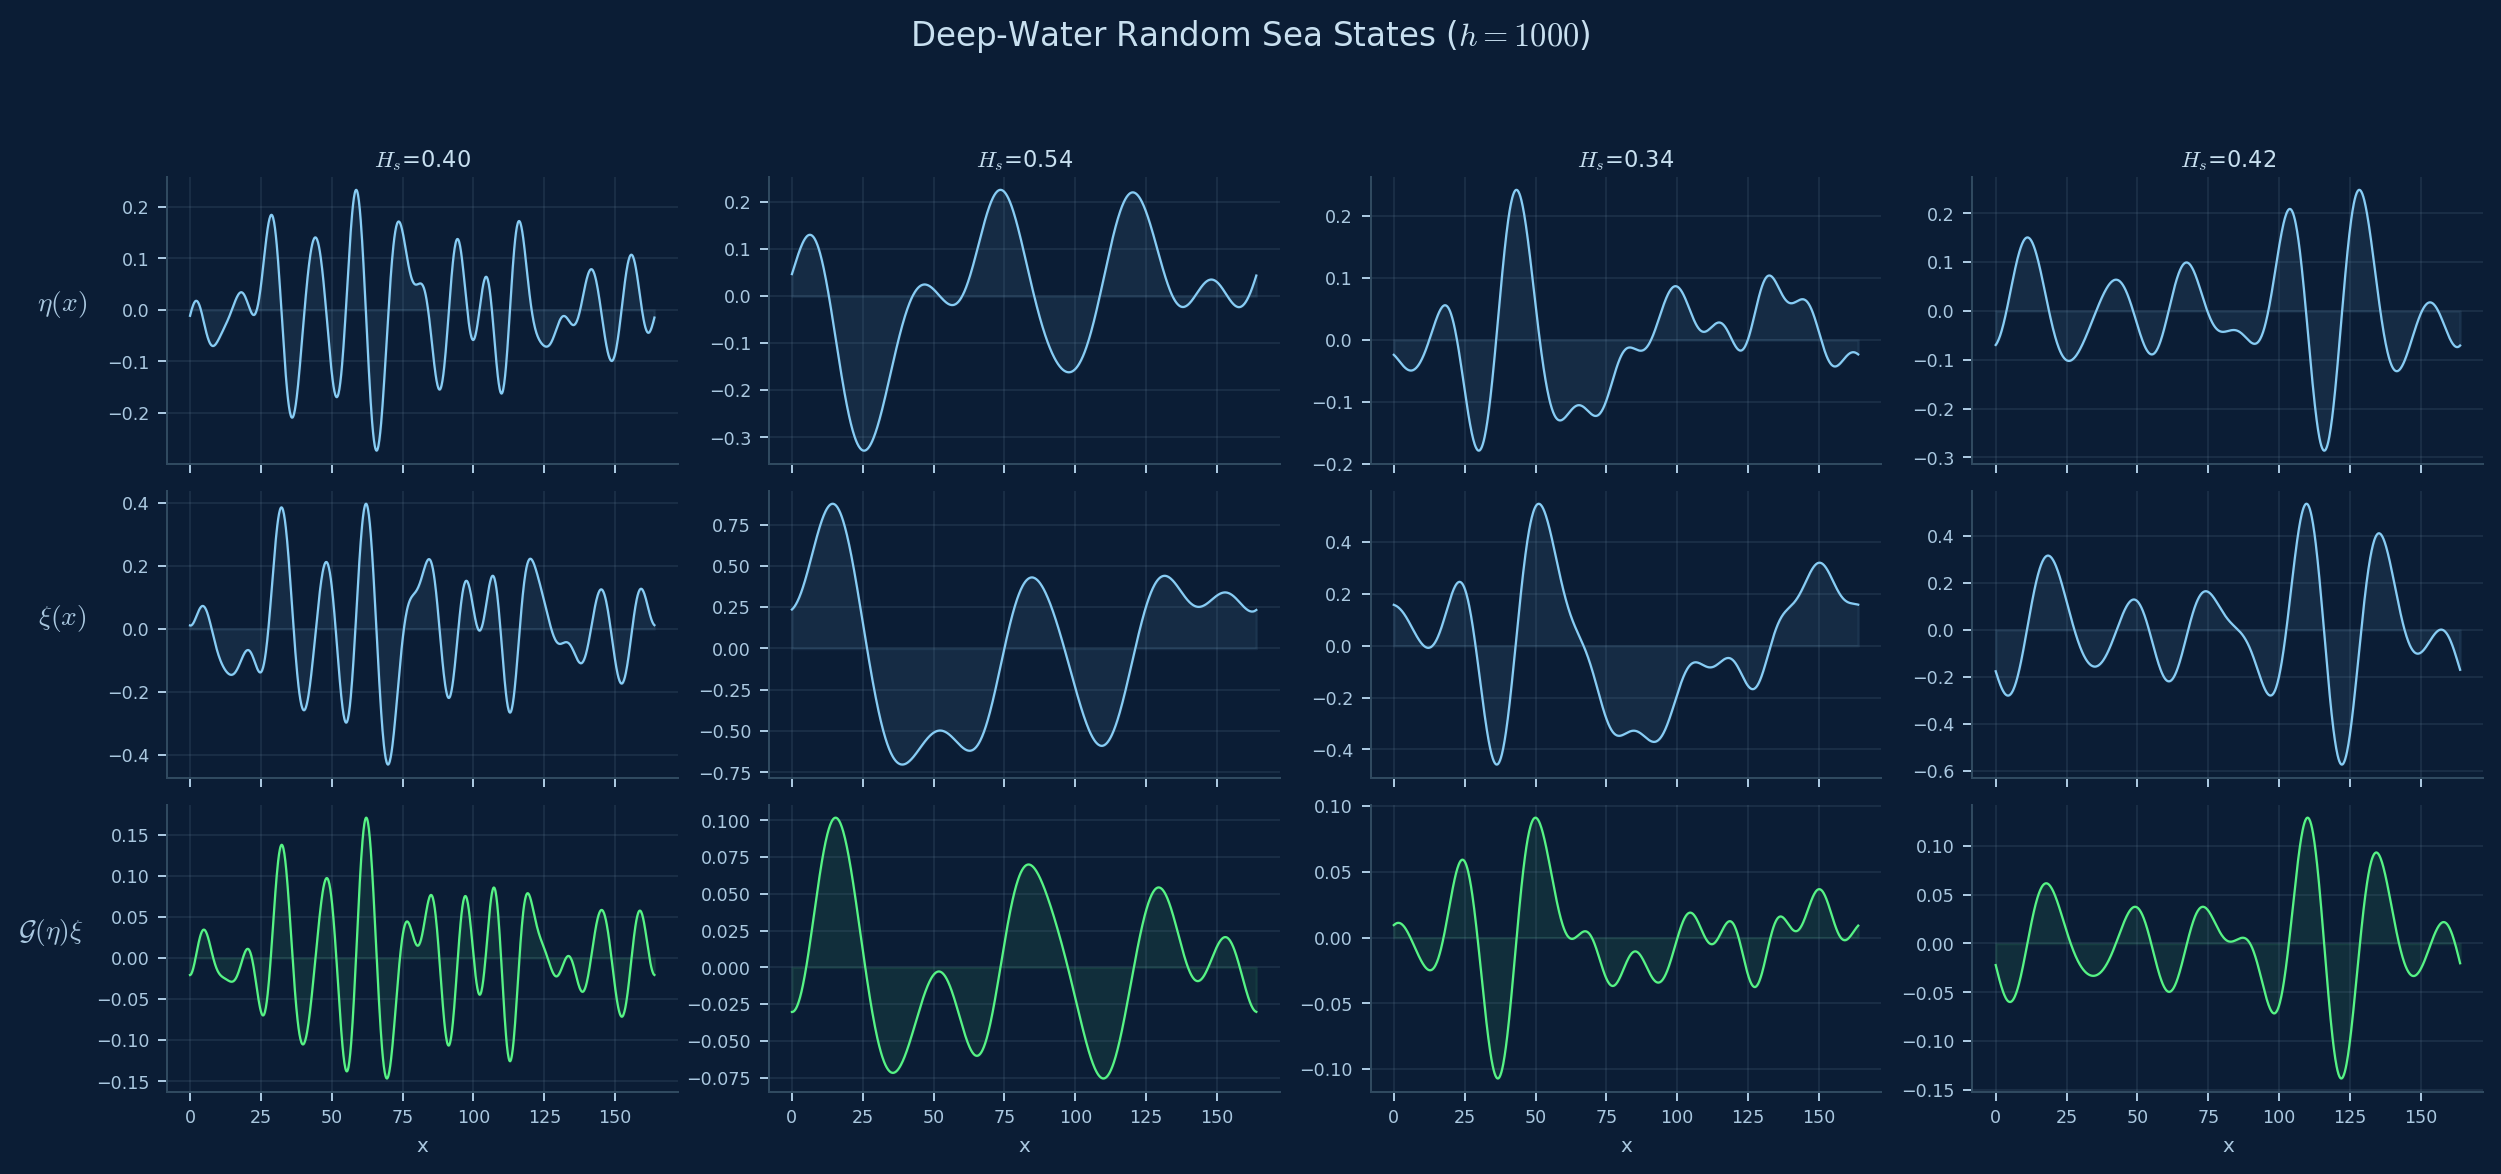
\includegraphics[width=\linewidth,height=0.85\textheight,keepaspectratio]{figures/random_sea_samples_1.png}
\end{frame}

% ============================================================
\begin{frame}{Random Sea Samples ($h = 1000$) (cont.)}
\centering
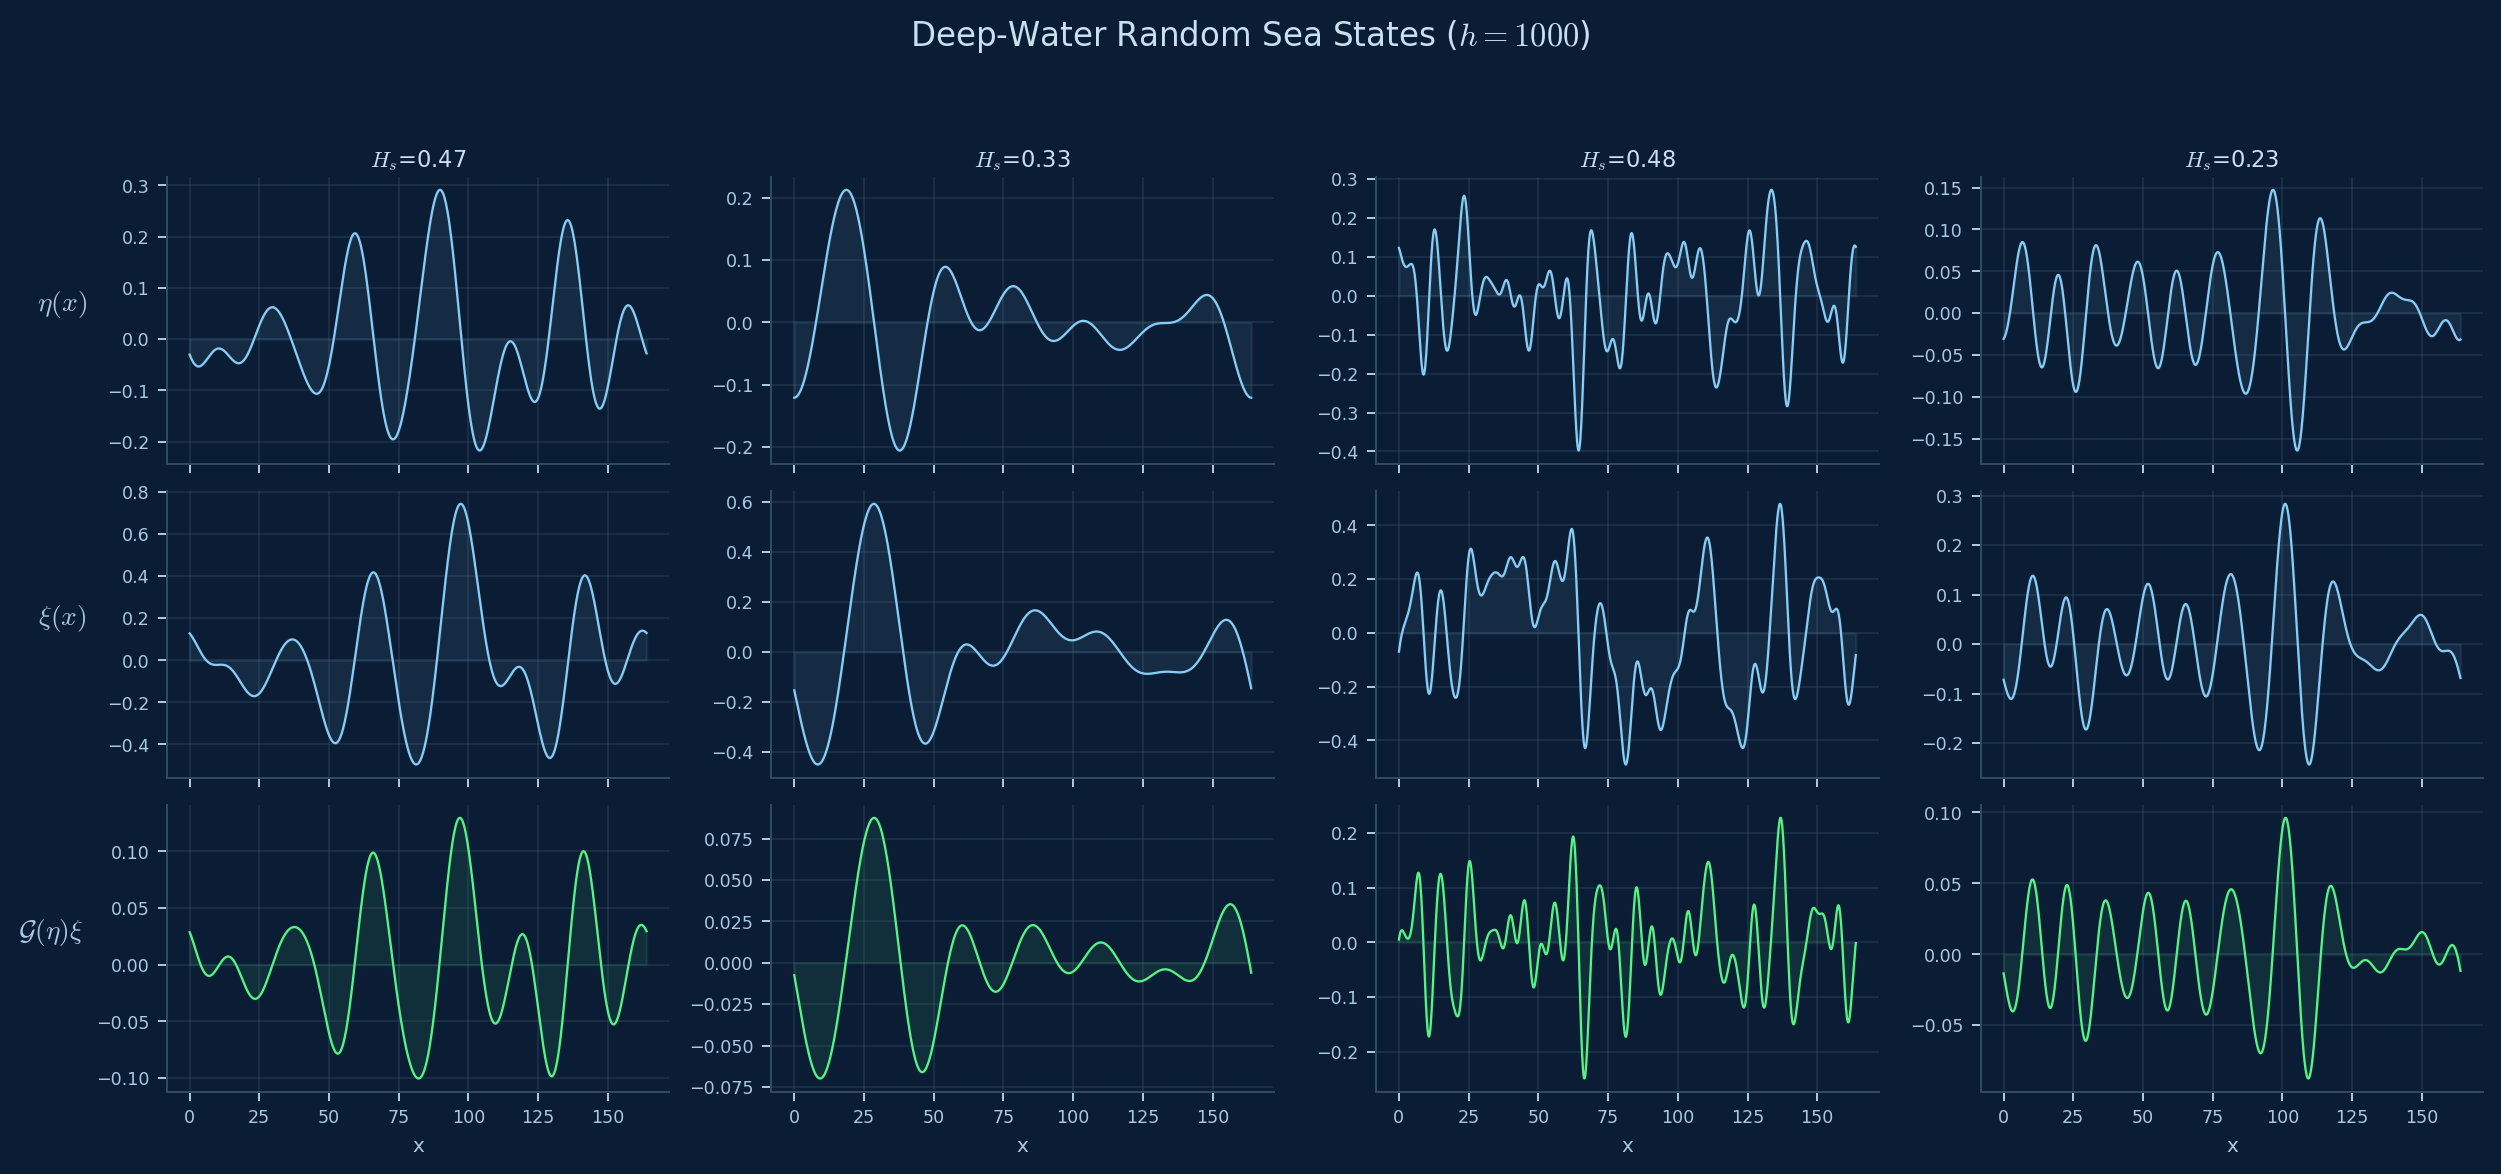
\includegraphics[width=\linewidth,height=0.85\textheight,keepaspectratio]{figures/random_sea_samples_2.png}
\end{frame}

% ============================================================
\begin{frame}{Tanaka Soliton Initial Conditions ($h = 1$)}
\centering
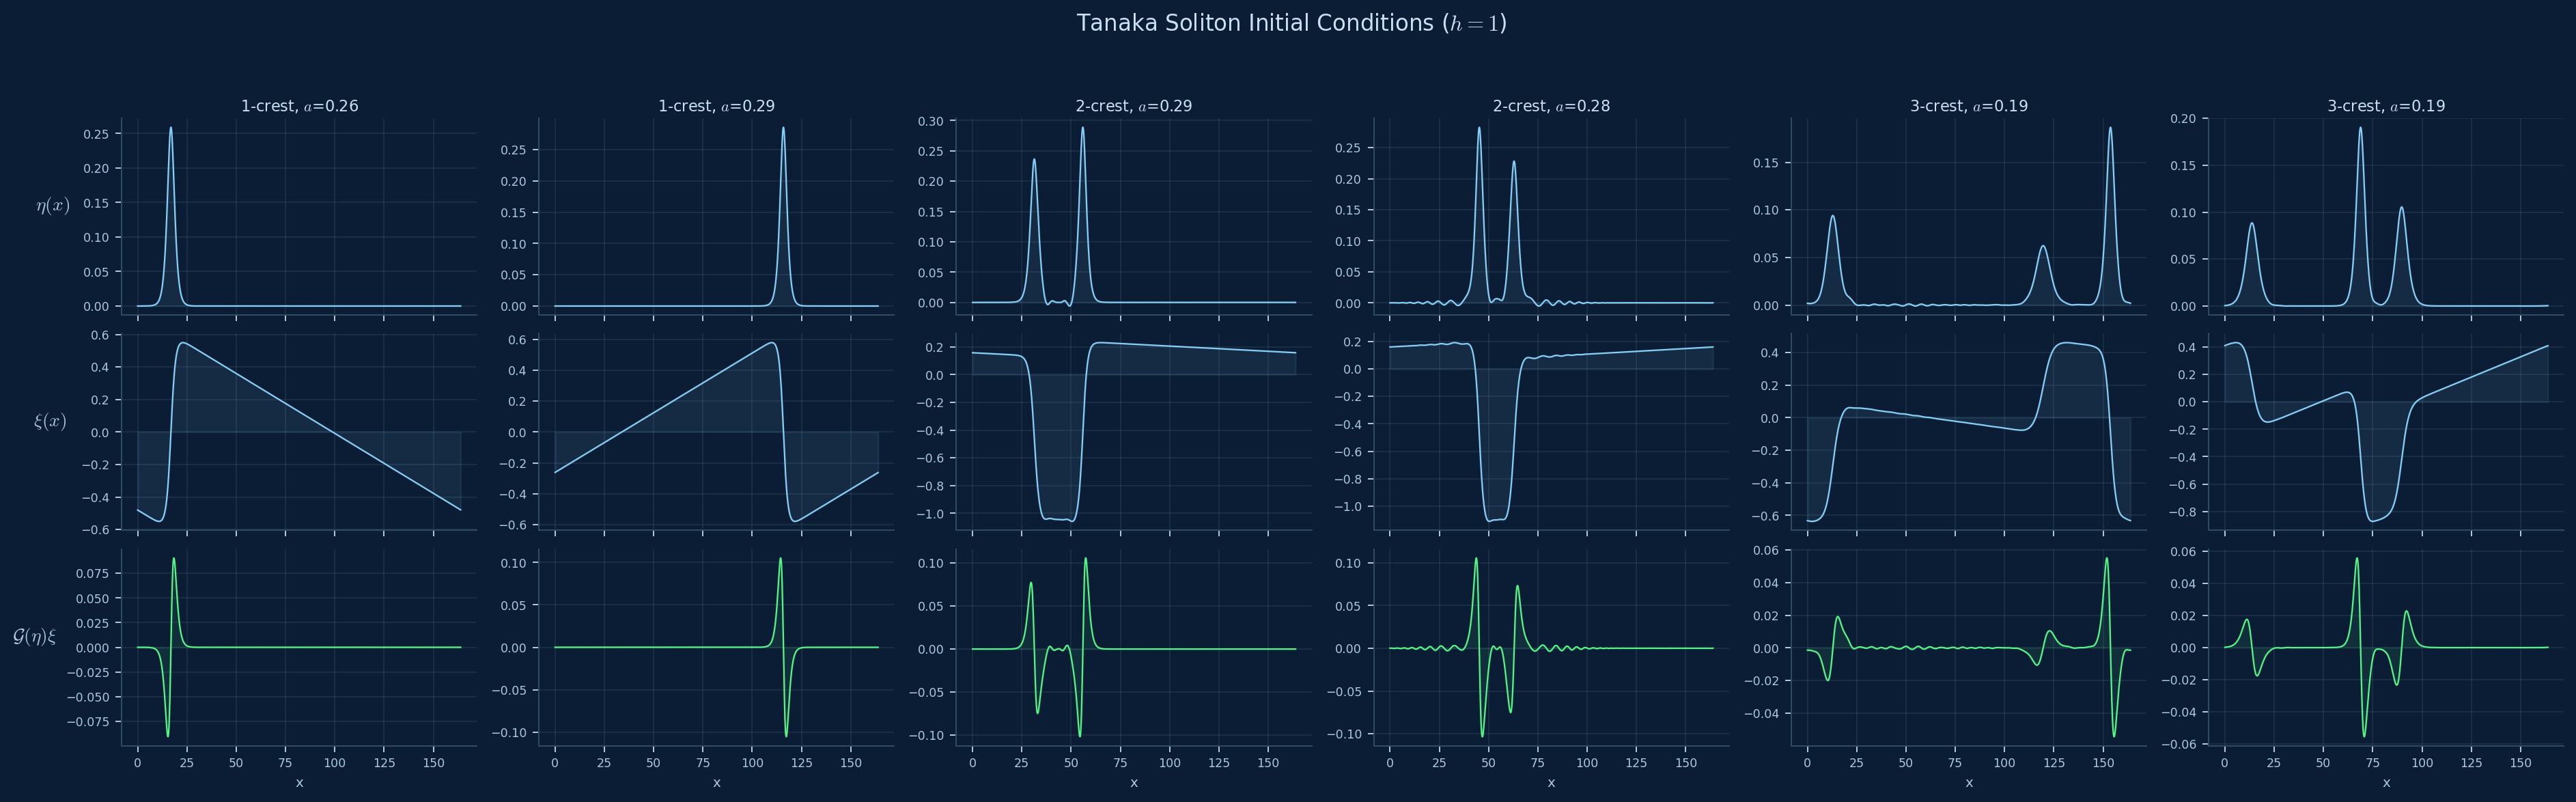
\includegraphics[width=\linewidth,height=0.85\textheight,keepaspectratio]{figures/tanaka_ics.png}
\end{frame}

% ============================================================
\begin{frame}{Single Soliton Trajectory ($h = 1$)}
\centering
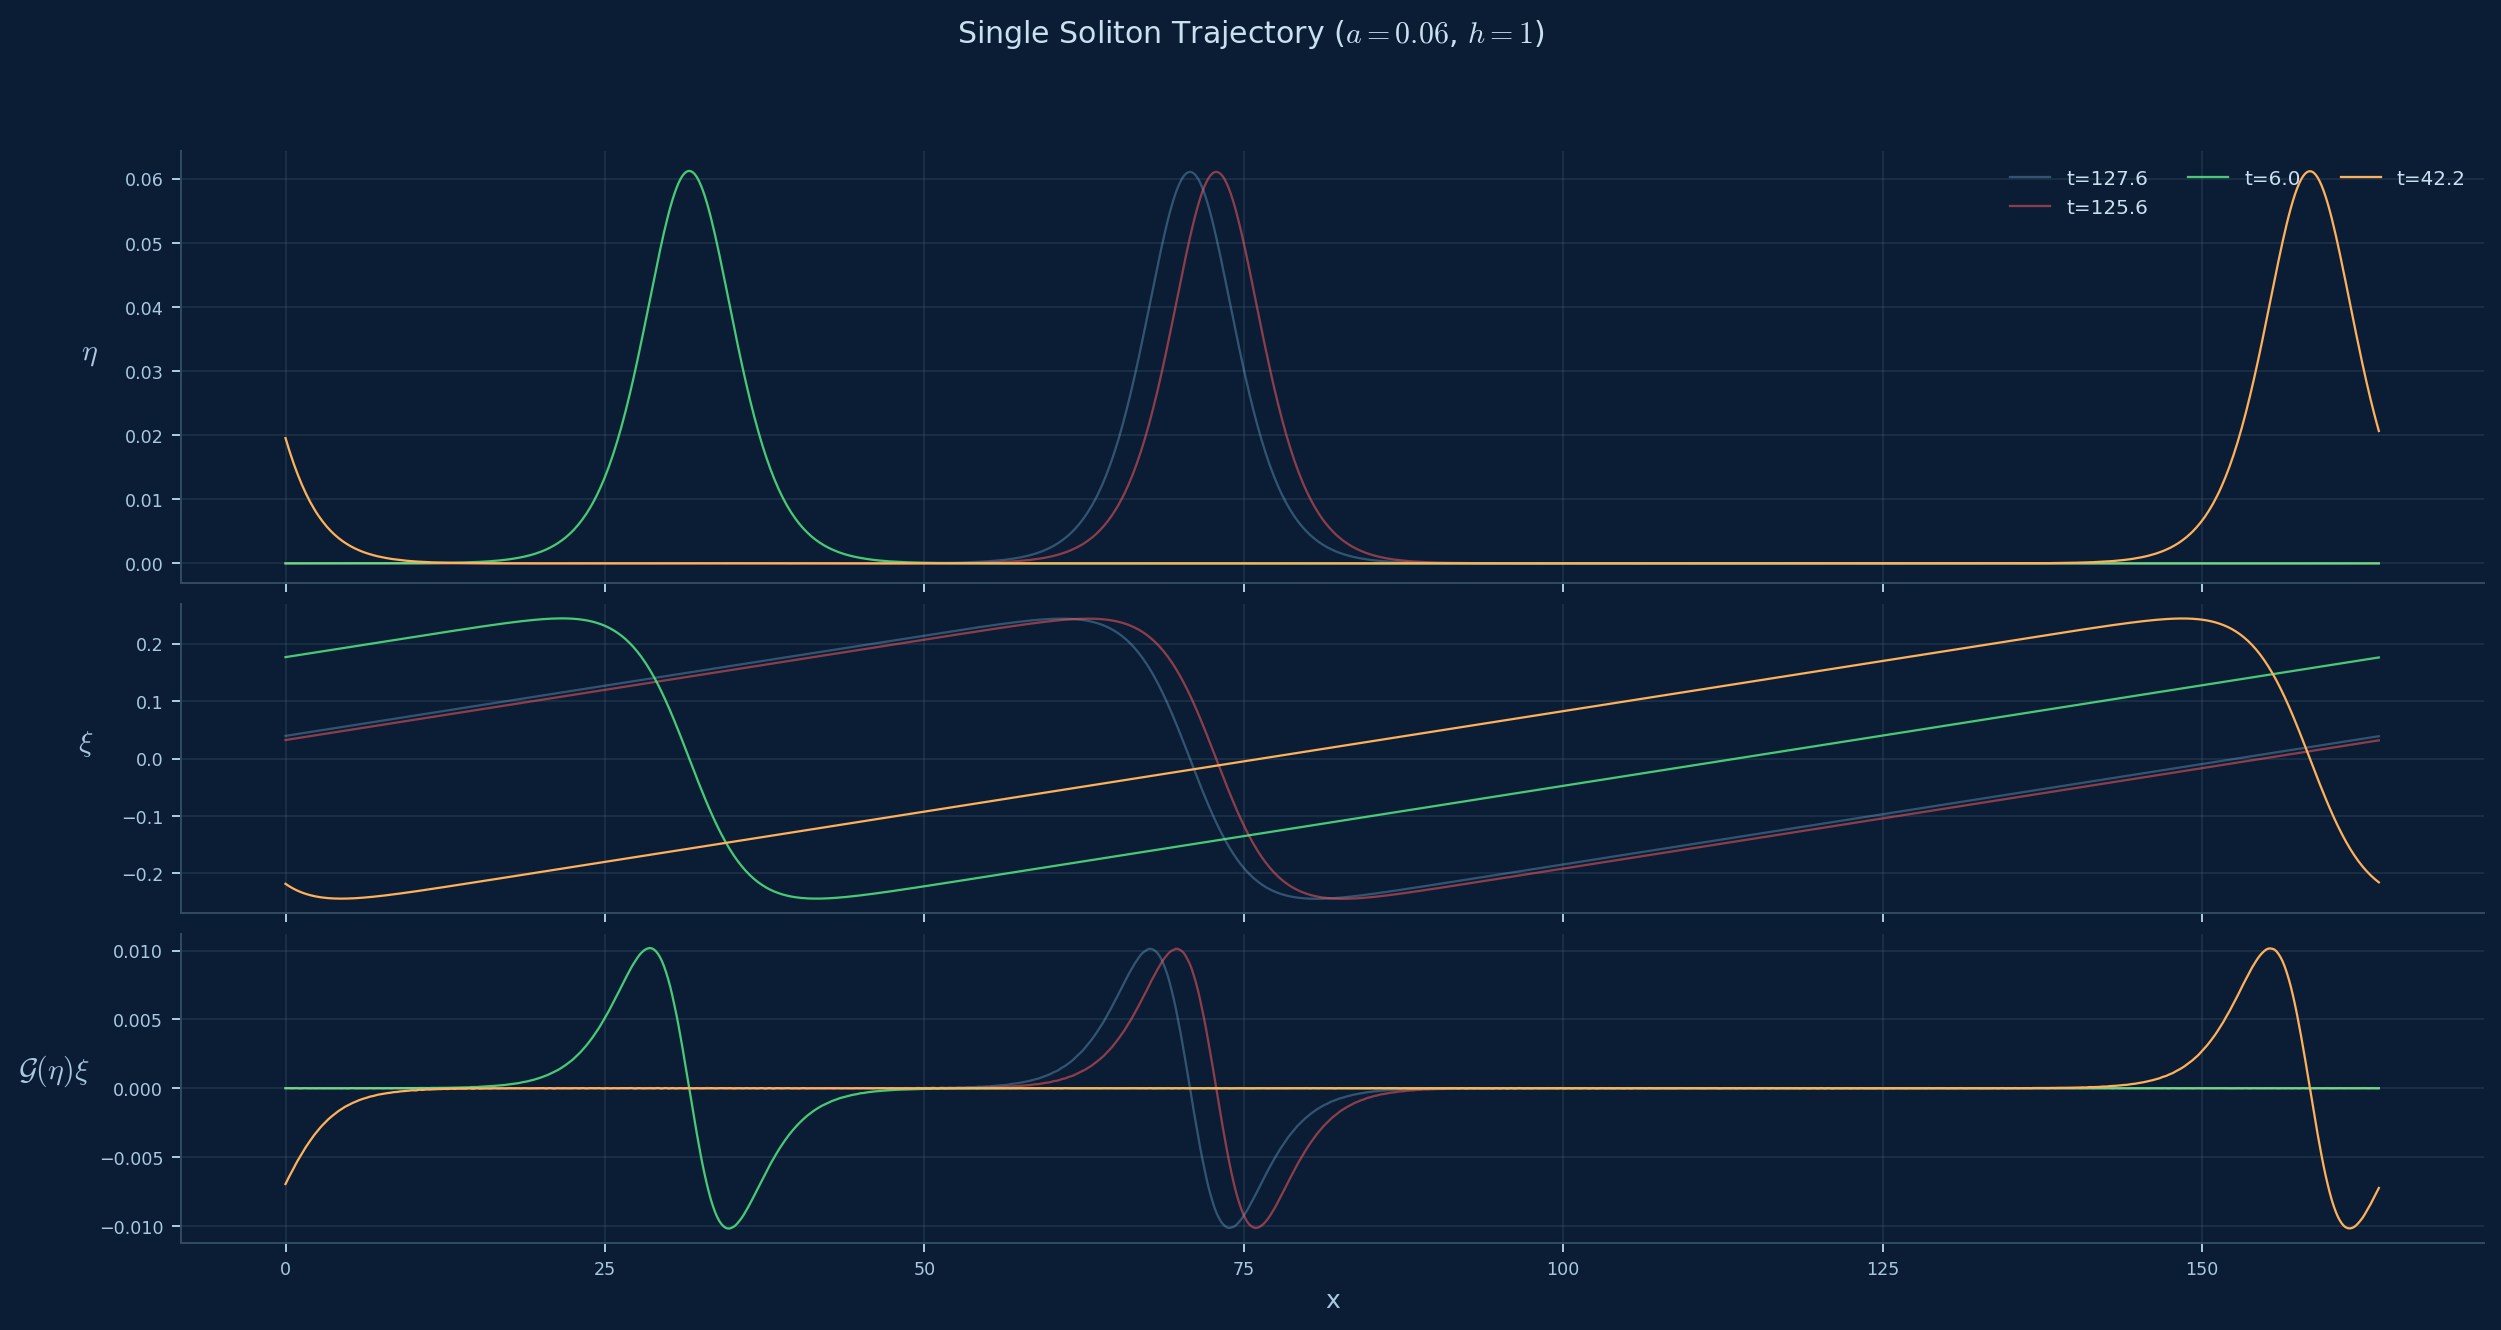
\includegraphics[width=\linewidth,height=0.85\textheight,keepaspectratio]{figures/tanaka_trajectory_1crest.png}
\end{frame}

% ============================================================
\begin{frame}{2-Crest Soliton Trajectory ($h = 1$)}
\centering
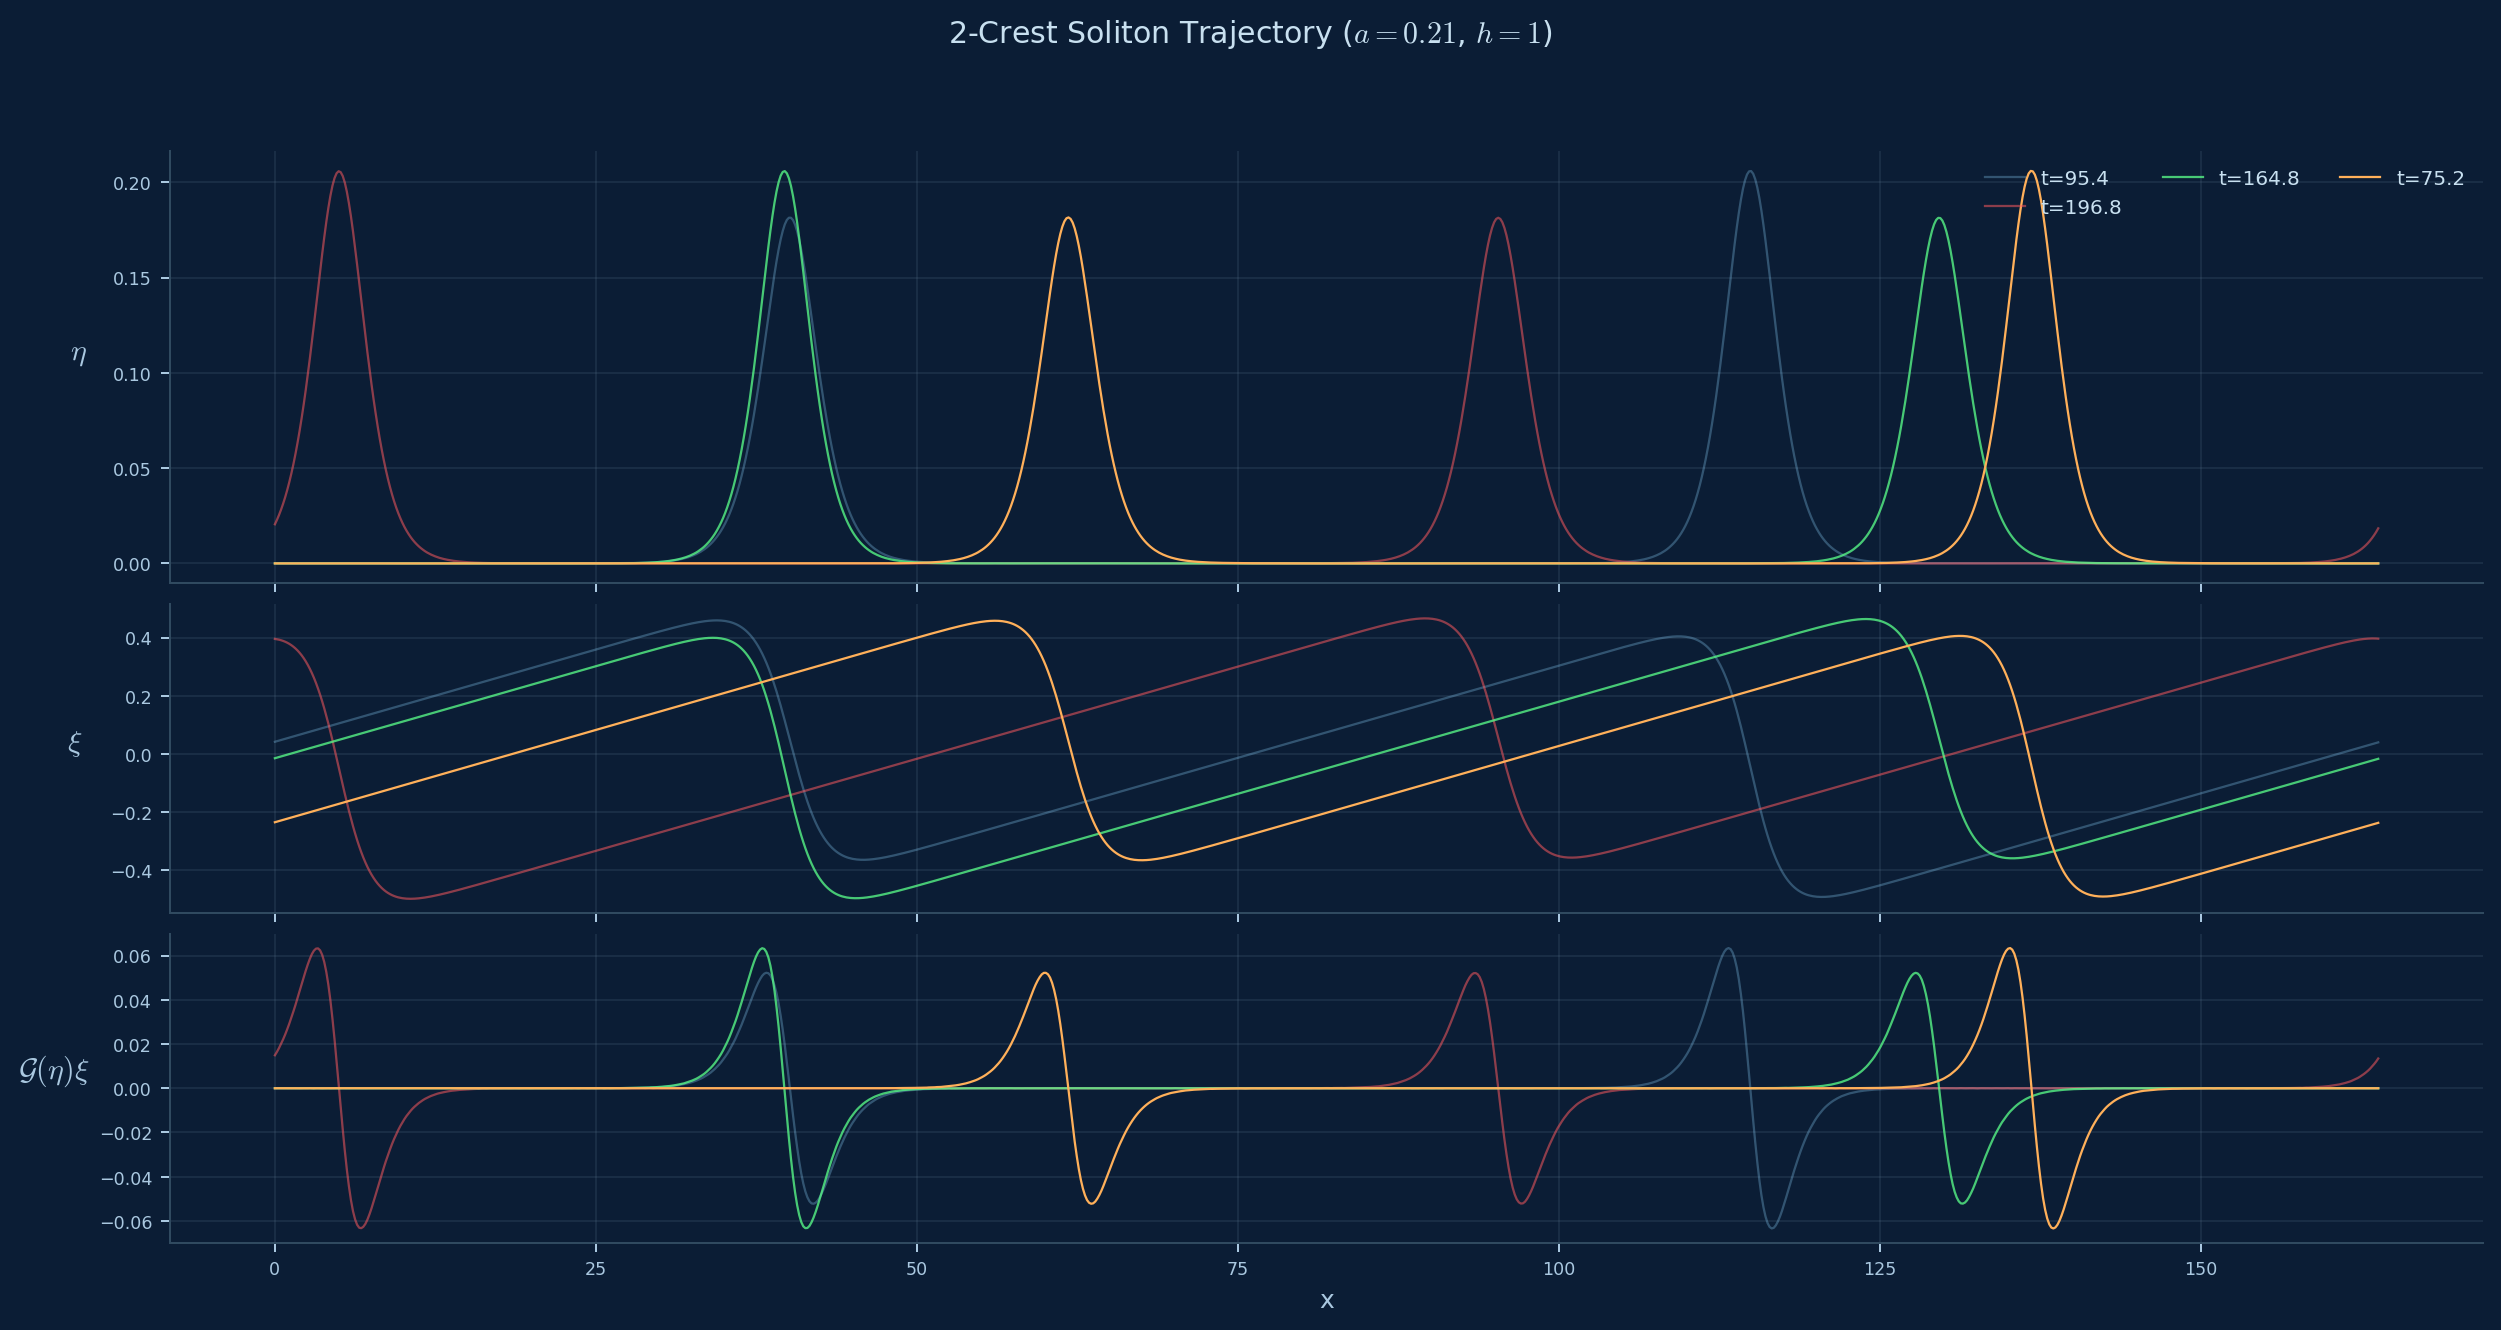
\includegraphics[width=\linewidth,height=0.85\textheight,keepaspectratio]{figures/tanaka_trajectory_2crest.png}
\end{frame}

% ============================================================
\begin{frame}{3-Crest Soliton Trajectory ($h = 1$)}
\centering
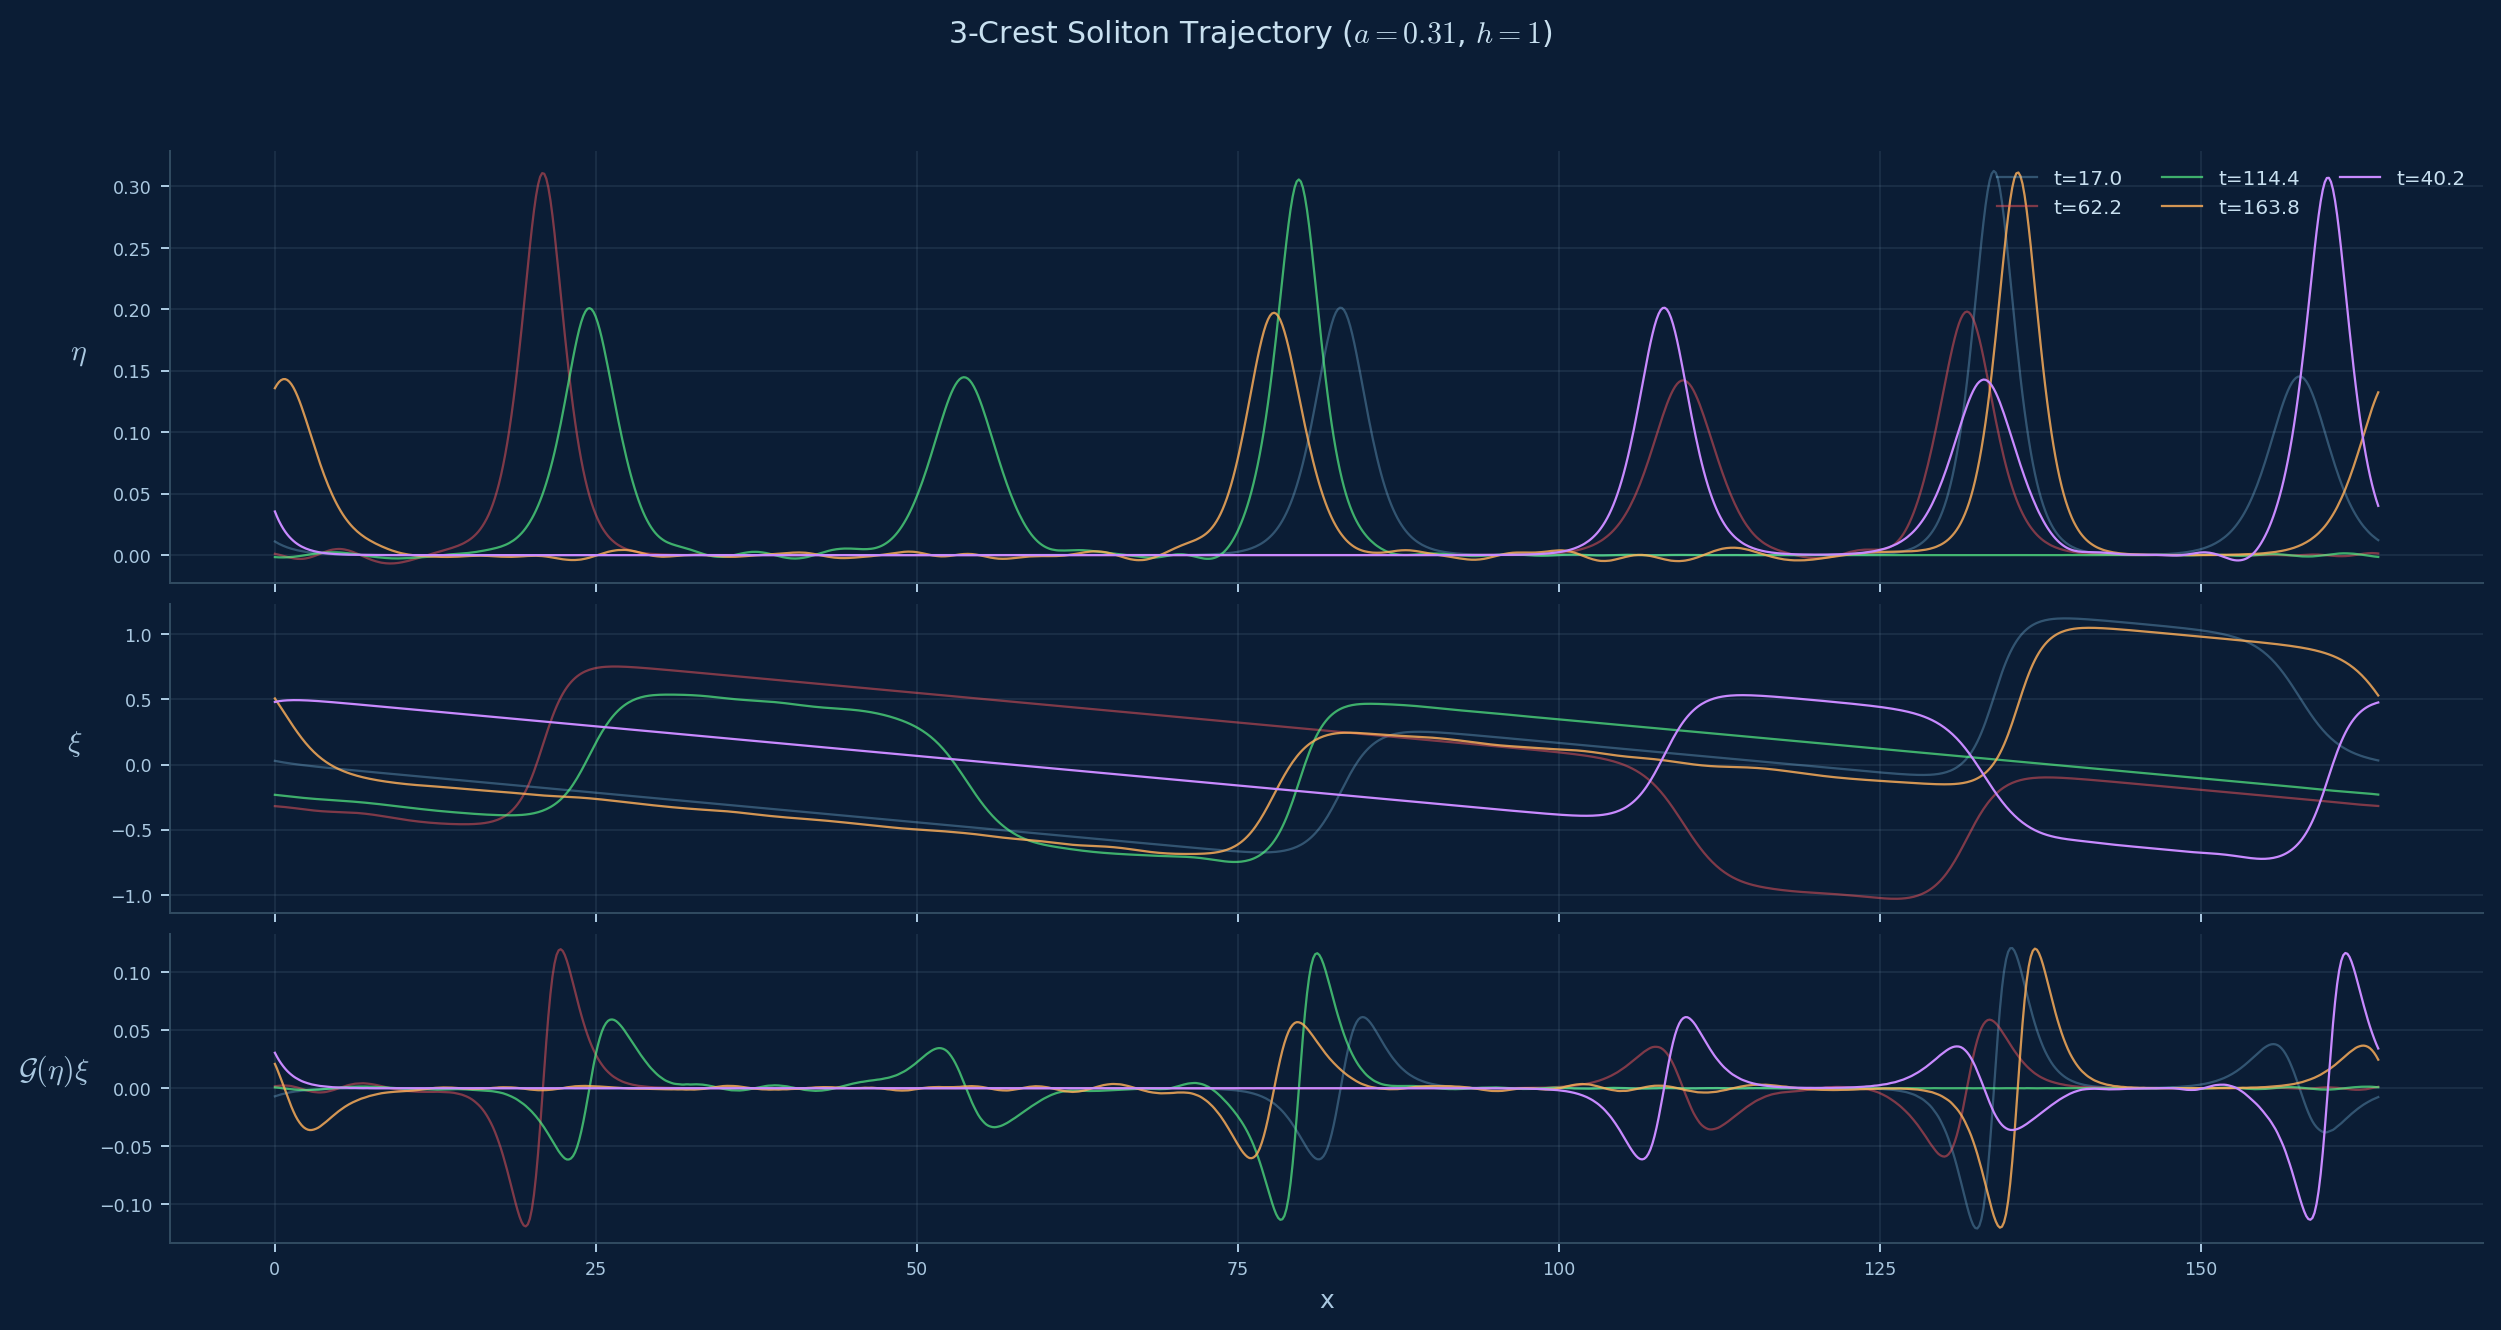
\includegraphics[width=\linewidth,height=0.85\textheight,keepaspectratio]{figures/tanaka_trajectory_3crest.png}
\end{frame}

% ============================================================
\section{FNO Architecture}

% ============================================================
\begin{frame}{Architecture Overview}

\begin{center}
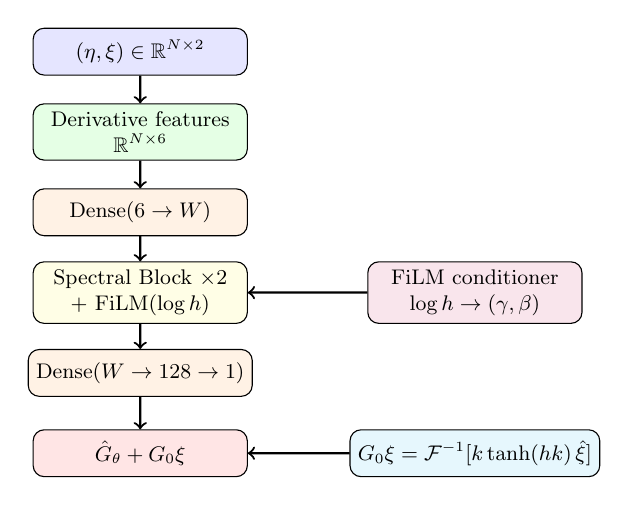
\begin{tikzpicture}[
  box/.style={draw, rounded corners, minimum width=3.2cm, minimum height=0.7cm, align=center, font=\small},
  arr/.style={->, thick},
  scale=0.85, transform shape
]
  \node[box, fill=blue!10] (input) at (0,0) {$(\eta, \xi) \in \R^{N \times 2}$};
  \node[box, fill=green!10] (deriv) at (0,-1.2) {Derivative features\\$\R^{N \times 6}$};
  \node[box, fill=orange!10] (proj) at (0,-2.4) {Dense$(6 \to W)$};
  \node[box, fill=yellow!10] (block) at (0,-3.6) {Spectral Block $\times 2$\\+ FiLM$(\log h)$};
  \node[box, fill=orange!10] (out) at (0,-4.8) {Dense$(W \to 128 \to 1)$};
  \node[box, fill=red!10] (sum) at (0,-6.0) {$\hat{G}_\theta + G_0\xi$};

  \node[box, fill=purple!10] (film) at (5,-3.6) {FiLM conditioner\\$\log h \to (\gamma, \beta)$};
  \node[box, fill=cyan!10] (baseline) at (5,-6.0) {$G_0\xi = \mathcal{F}^{-1}[k\tanh(hk)\,\hat\xi]$};

  \draw[arr] (input) -- (deriv);
  \draw[arr] (deriv) -- (proj);
  \draw[arr] (proj) -- (block);
  \draw[arr] (block) -- (out);
  \draw[arr] (out) -- (sum);
  \draw[arr] (film) -- (block);
  \draw[arr] (baseline) -- (sum);
\end{tikzpicture}
\end{center}

\textbf{147k parameters.} Modes $M = 32$, width $W = 32$, 2 spectral blocks.
\end{frame}

% ============================================================
\begin{frame}{Key Design Choices}

\textbf{1. Linear DNO baseline (residual learning):}
\[
  \hat\Gop_\theta(\eta,\xi;h) = \underbrace{G_0(k;h)\,\xi}_{\text{linear estimate}} + \underbrace{f_\theta(\eta, \xi, \log h)}_{\text{learned nonlinear residual}}
\]
where $G_0(k;h) = k\,\tanh(hk)$ is the linear DNO symbol applied as a Fourier multiplier.

The network only learns $\Gop - G_0\xi$, which is $O(\eta)$.

\pause

\textbf{2. FiLM depth conditioning:}
\[
  x^{(\ell)} \leftarrow (1 + \gamma^{(\ell)})\,x^{(\ell)} + \beta^{(\ell)},
  \quad (\gamma, \beta) = \text{MLP}(\log h).
\]
A single network handles all depths via per-layer affine modulation.


\end{frame}
\begin{frame}{Key Design Choices}
\textbf{3. Spectral convolutions} with weight normalization: learned complex weights on the first 32 Fourier modes, with per-mode Frobenius normalization and scalar gains.

\pause

\textbf{4. Derivative features:} finite-difference $\eta_x, \xi_x, \eta_{xx}, \xi_{xx}$ concatenated to input ($2 \to 6$ channels).
\end{frame}

% ============================================================
\begin{frame}{Training Details}

\begin{columns}[T]
\begin{column}{0.48\textwidth}
\textbf{Optimizer:} AdamW\\
\textbf{Learning rate:} $5 \times 10^{-4}$ with cosine decay\\
\textbf{Weight decay:} $10^{-4}$\\
\textbf{Batch size:} 128\\
\textbf{Epochs:} 40\\
\textbf{Split:} 160k train / 20k val / 20k test


\textbf{Loss:} Sobolev loss
\[
  \mathcal{L} = \relltwo(\hat y, y) + \relltwo_{\!H^1}(\hat y, y),
\]
where $\relltwo_{H^1}$ weights the Fourier coefficients by $\sqrt{1 + n^2}$.


\textbf{Normalization:} divide features by $|\cdot|_\infty$:
\begin{itemize}
  \item $\eta$: $\div\; 0.75$
  \item $\xi$: $\div\; 1.52$
  \item $\Gop\xi$: $\div\; 0.46$
\end{itemize}
\end{column}

\begin{column}{0.48\textwidth}
\textbf{Training curve:}


\begin{tabular}{rcc}
\toprule
Epoch & Train & Val \\
\midrule
1  & 1.078  & 0.175 \\
10 & 0.087  & 0.057 \\
20 & 0.015  & 0.013 \\
30 & 0.008  & 0.008 \\
37 & 0.008  & \textbf{0.0074} \\
40 & 0.007  & 0.007 \\
\bottomrule
\end{tabular}


Best checkpoint: epoch 37, val loss $= 0.0074$.

\end{column}
\end{columns}
\end{frame}

% ============================================================
\section{Generalization Results}

% ============================================================
\begin{frame}{Motivation: Why Depth Matters}

An FNO trained only on Tanaka solitons ($h = 1$) fails to generalize:

\begin{itemize}
  \item The linear DNO symbol $G_0(k) = k\,\tanh(hk)$ changes qualitatively with depth
  \item Deep water ($h \to \infty$): $G_0(k) \to |k|$
  \item Shallow water ($h \to 0$): $G_0(k) \to hk^2$
  \item A single-depth model bakes in the wrong dispersion relation
\end{itemize}

\pause

\textbf{Solution:}
\begin{enumerate}
  \item Include depth as a FiLM-conditioned input ($\log h$)
  \item Provide the linear baseline $G_0\xi$ analytically --- the network only learns the nonlinear correction
  \item Train on two depth regimes: $h = 1$ (Tanaka) and $h = 1000$ (random sea)
\end{enumerate}

The linear baseline alone achieves $\sim$11\% error on the Tanaka data. The learned residual brings this down to $\sim$0.1\%.
\end{frame}

% ============================================================
\begin{frame}{Pointwise Evaluation: Tanaka Solitons ($h = 1$)}

\textbf{Test set:} 5,000 Tanaka soliton snapshots (held out from training).

\pause

\begin{center}
\begin{tabular}{lc}
\toprule
Metric & Value \\
\midrule
Mean $\relltwo$   & $\mathbf{0.0012}$ \\
Median $\relltwo$ & $0.0007$ \\
$p_{95}$ $\relltwo$ & $0.0033$ \\
$p_{99}$ $\relltwo$ & $0.0060$ \\
\bottomrule
\end{tabular}
\end{center}


Median error is $0.07\%$. Even the 99th percentile stays below $0.6\%$.

The FNO captures the full nonlinear DNO across 1--3 crest solitons with amplitudes up to $0.35$.
\end{frame}

% ============================================================
\begin{frame}{Tanaka Soliton Eval: Samples \& Error Distribution}
\centering
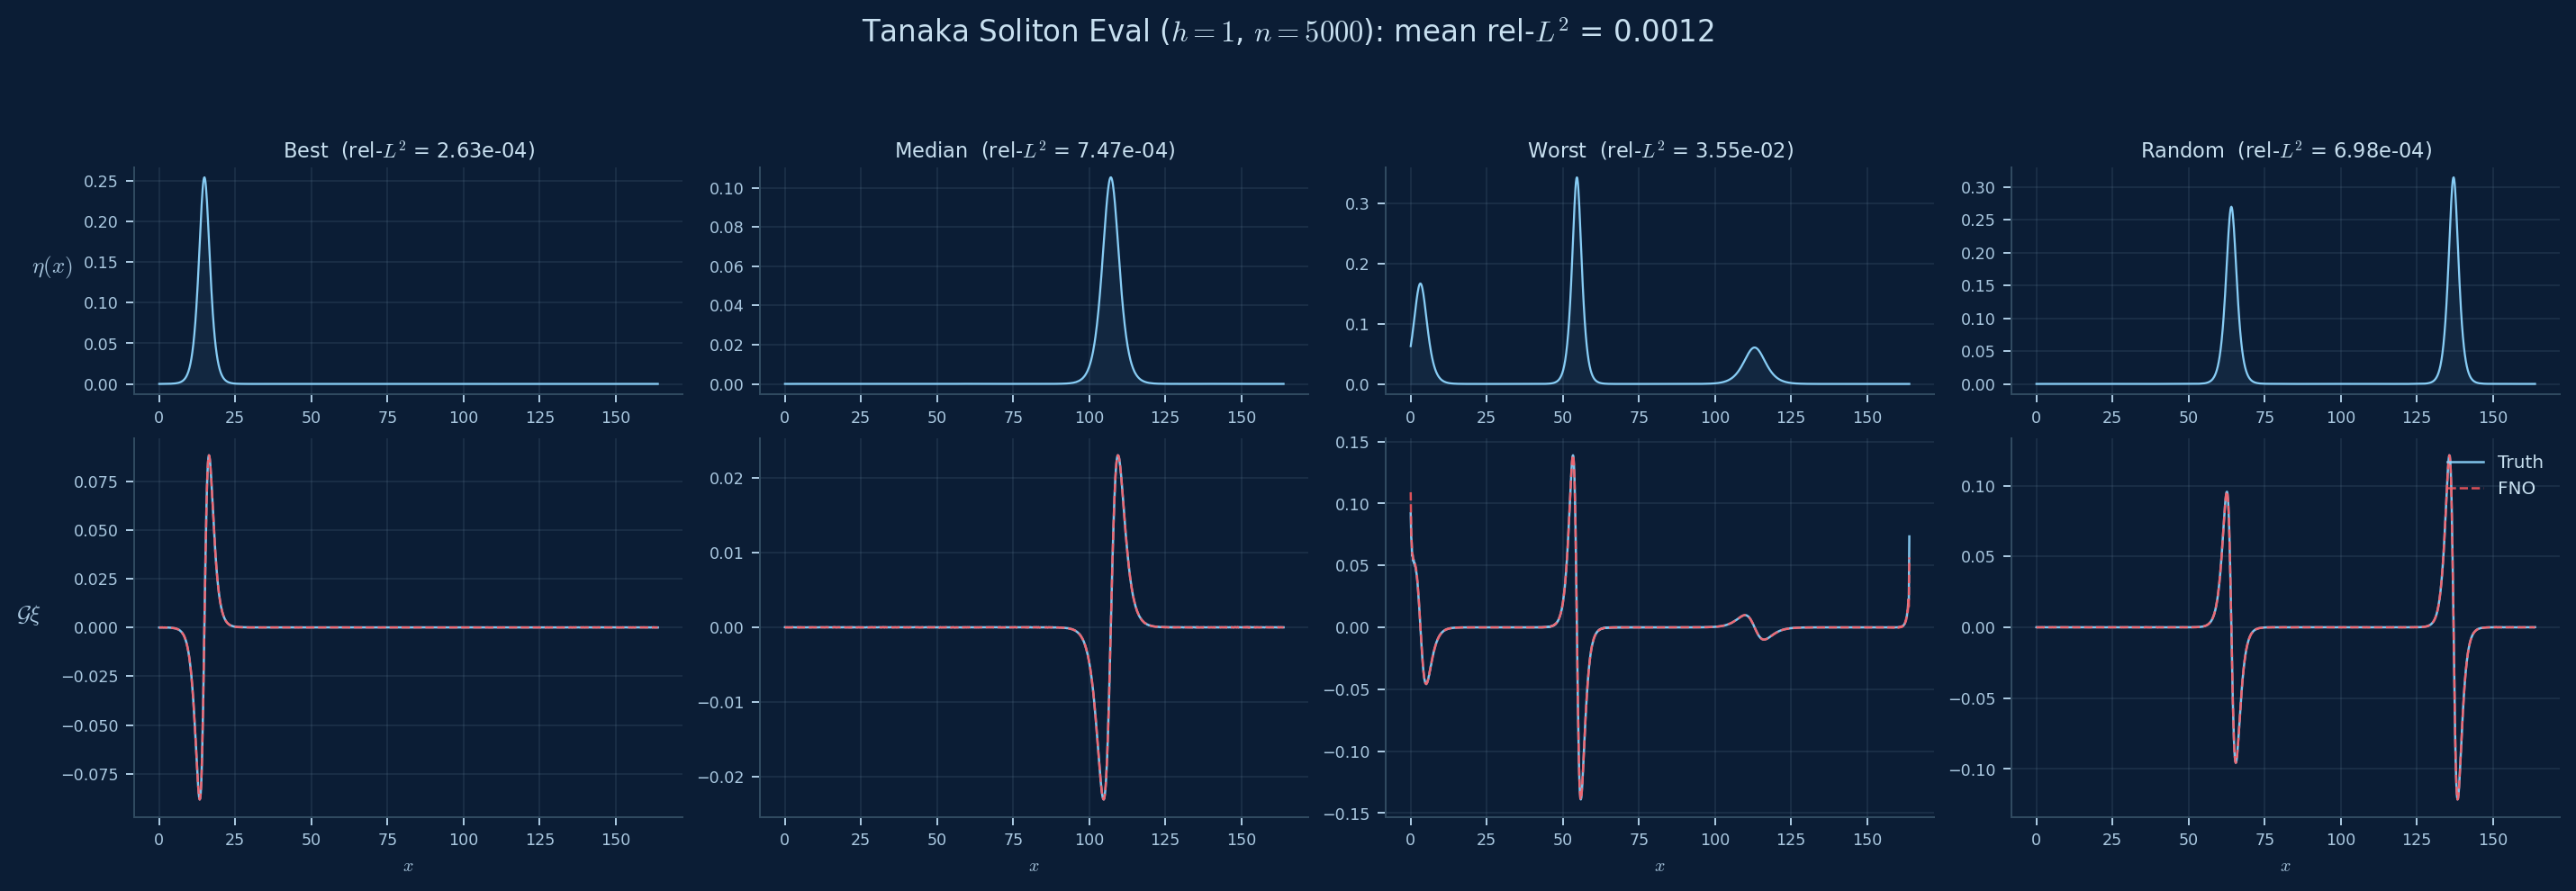
\includegraphics[width=\linewidth,height=0.42\textheight,keepaspectratio]{figures/eval_tanaka_samples.png}
\vspace{0.2em}
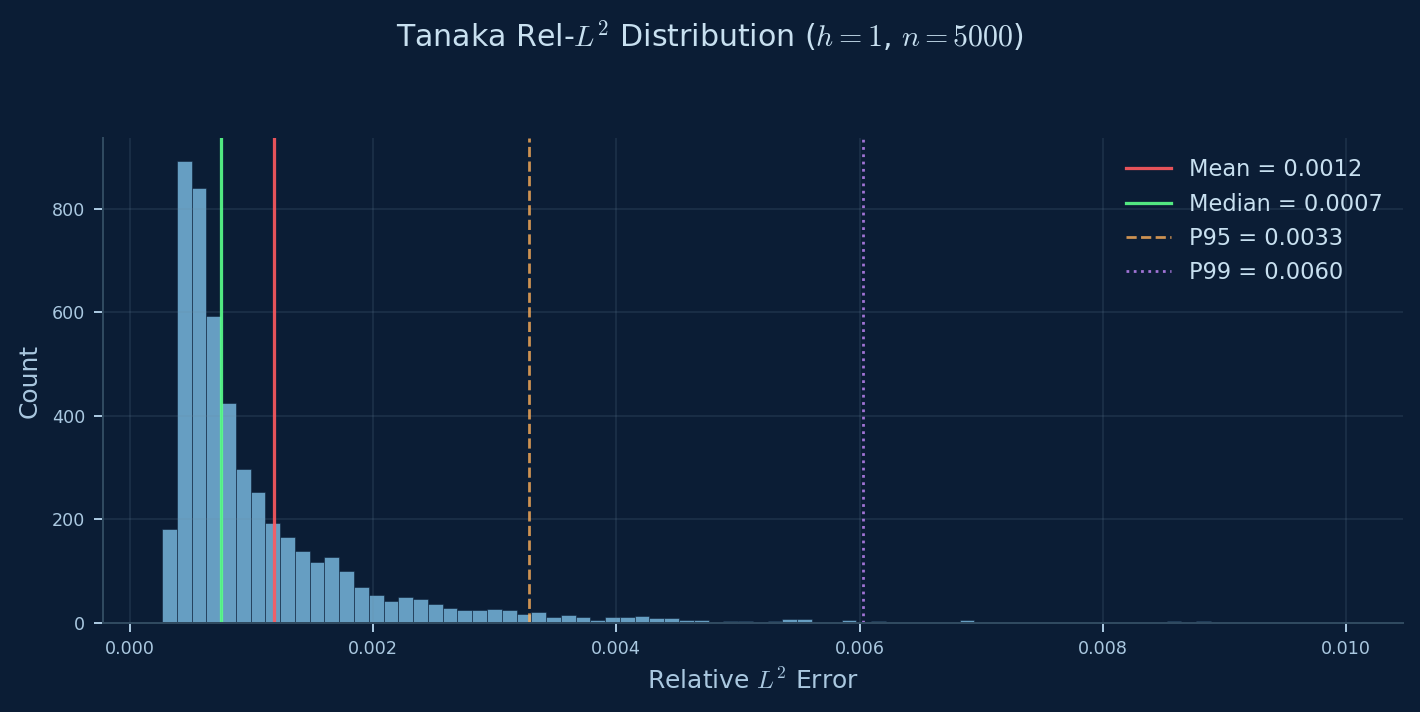
\includegraphics[width=0.75\linewidth,height=0.42\textheight,keepaspectratio]{figures/eval_tanaka_hist.png}
\end{frame}

% ============================================================
\begin{frame}{Pointwise Evaluation: DNO Dataset Solitons ($h = 1$)}

\textbf{Test set:} 30,030 soliton snapshots from Philippe's Google drive data (not used in training). Amplitudes up to $a = 0.92$, including multi-crest interactions.


\begin{center}
\begin{tabular}{lc}
\toprule
Metric & Value \\
\midrule
Mean $\relltwo$   & $\mathbf{0.0064}$ \\
Median $\relltwo$ & $0.0062$ \\
Std $\relltwo$    & $0.0098$ \\
$p_{95}$ $\relltwo$ & $0.0168$ \\
$p_{99}$ $\relltwo$ & $0.0512$ \\
\bottomrule
\end{tabular}
\end{center}


Median error stays below $0.7\%$ across 30k independent soliton samples, including amplitudes well beyond the training range ($a \leq 0.35$). The 99th percentile at $5.1\%$ shows graceful degradation on the most extreme cases.
\end{frame}

% ============================================================
\begin{frame}{DNO Dataset Soliton Eval: Samples \& Error Distribution}
\centering
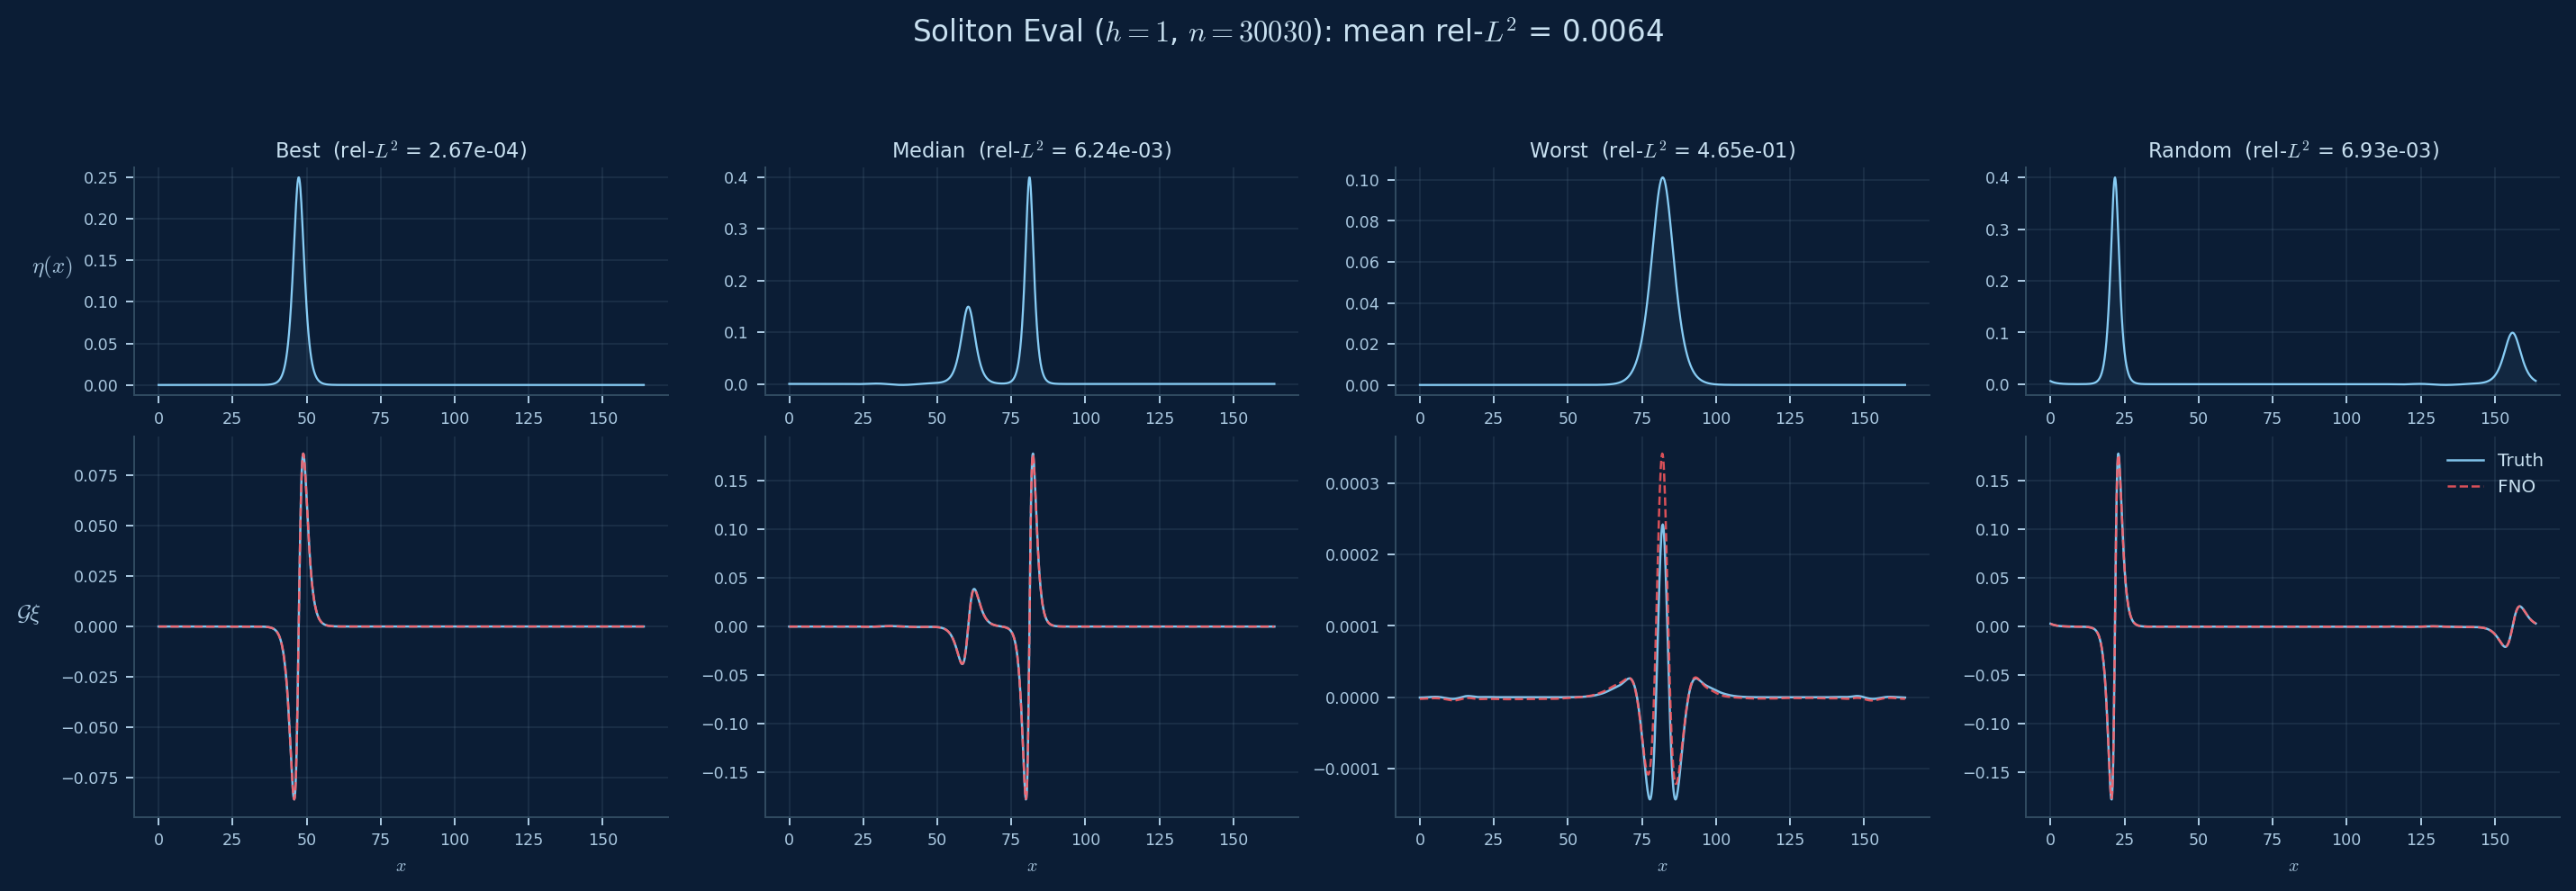
\includegraphics[width=\linewidth,height=0.42\textheight,keepaspectratio]{figures/eval_soliton_samples.png}
\vspace{0.2em}
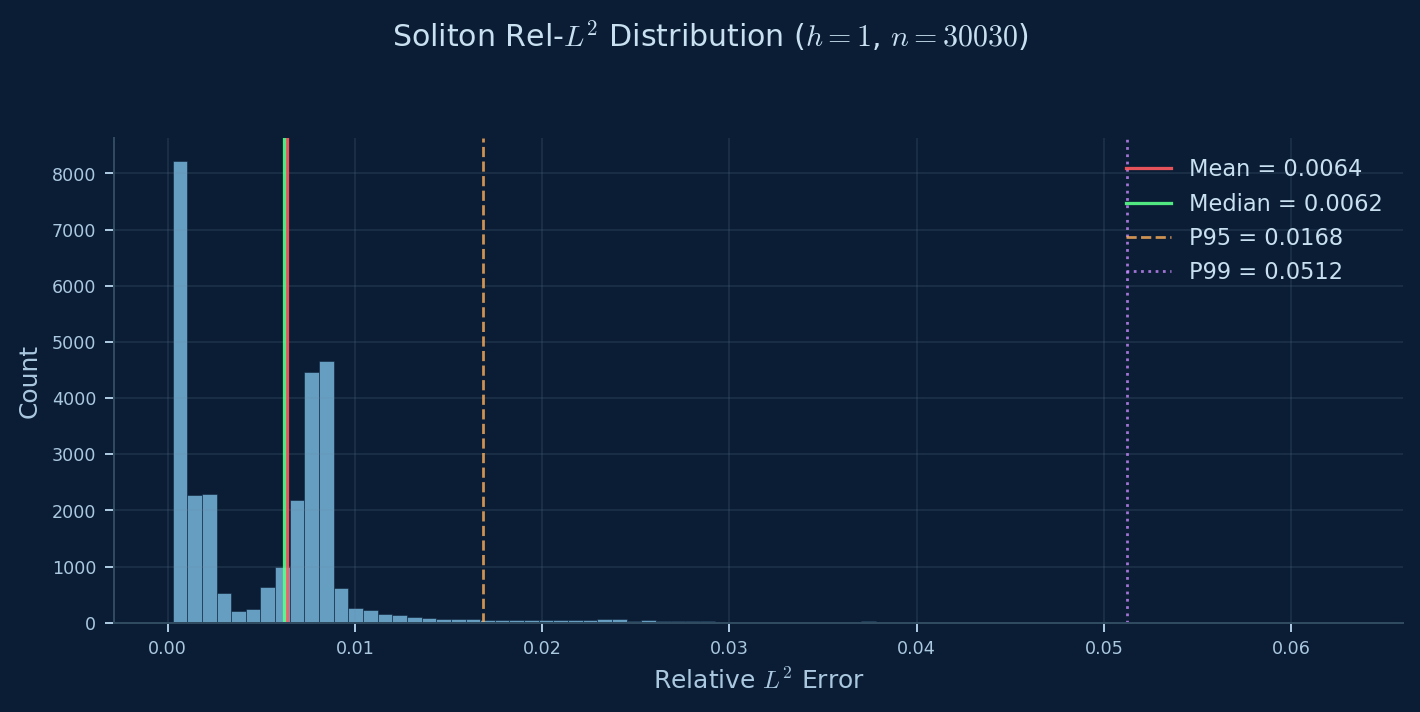
\includegraphics[width=0.75\linewidth,height=0.42\textheight,keepaspectratio]{figures/eval_soliton_hist.png}
\end{frame}

% ============================================================
\begin{frame}{Generalization to Stokes Waves}

\textbf{Not in training data.} Generated ad-hoc from 5th-order Stokes theory.

\pause

\begin{columns}[T]
\begin{column}{0.48\textwidth}
\textbf{Deep water} ($h = 1000$, 30 samples):

\begin{center}
\begin{tabular}{lc}
\toprule
Metric & Value \\
\midrule
Mean $\relltwo$   & $\mathbf{4.7 \times 10^{-4}}$ \\
Median $\relltwo$ & $3.0 \times 10^{-4}$ \\
\bottomrule
\end{tabular}
\end{center}

Wavenumbers $n_0 \in \{4, 6, 8, 10, 14, 20\}$, amplitudes $a_0 \in [0.01, 0.1]$, steepness $\varepsilon = k_0 a_0 < 0.3$.
\end{column}

\begin{column}{0.48\textwidth}
\textbf{Finite depth} ($h = 1$, 28 samples):

\begin{center}
\begin{tabular}{lc}
\toprule
Metric & Value \\
\midrule
Mean $\relltwo$   & $\mathbf{0.031}$ \\
Median $\relltwo$ & $0.024$ \\
\bottomrule
\end{tabular}
\end{center}

Finite-depth Stokes (Zhao \& Liu coefficients).
Higher error at large steepness ($\varepsilon > 0.04$).
\end{column}
\end{columns}

\pause

\textbf{Key:} The FNO generalizes from random sea training data to structured Stokes waves at both depths, despite never seeing Stokes profiles during training.
\end{frame}

% ============================================================
\begin{frame}{Stokes Eval: Deep Water ($h = 1000$)}
\centering
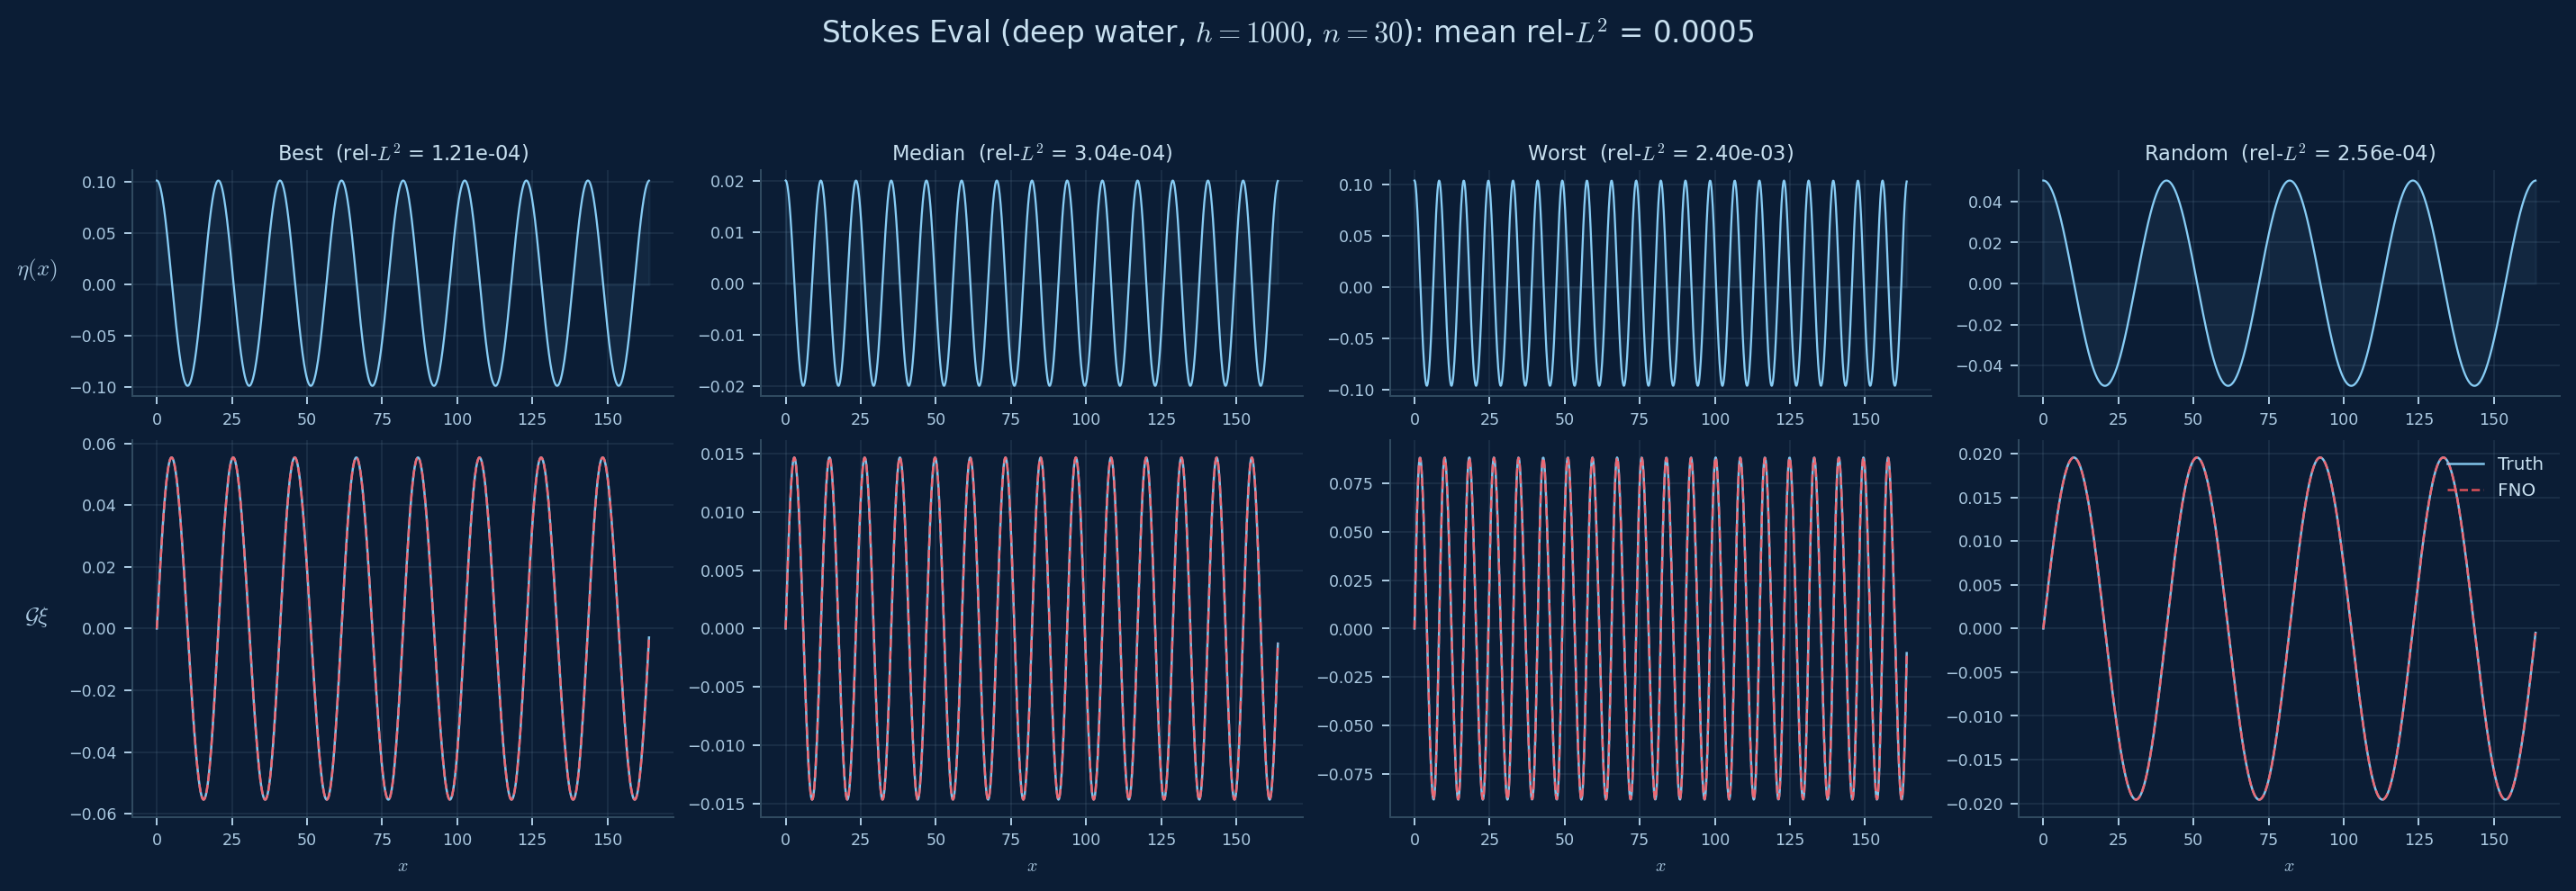
\includegraphics[width=\linewidth,height=0.85\textheight,keepaspectratio]{figures/eval_stokes_deep_samples.png}
\end{frame}

% ============================================================
\begin{frame}{Stokes Eval: Finite Depth ($h = 1$)}
\centering
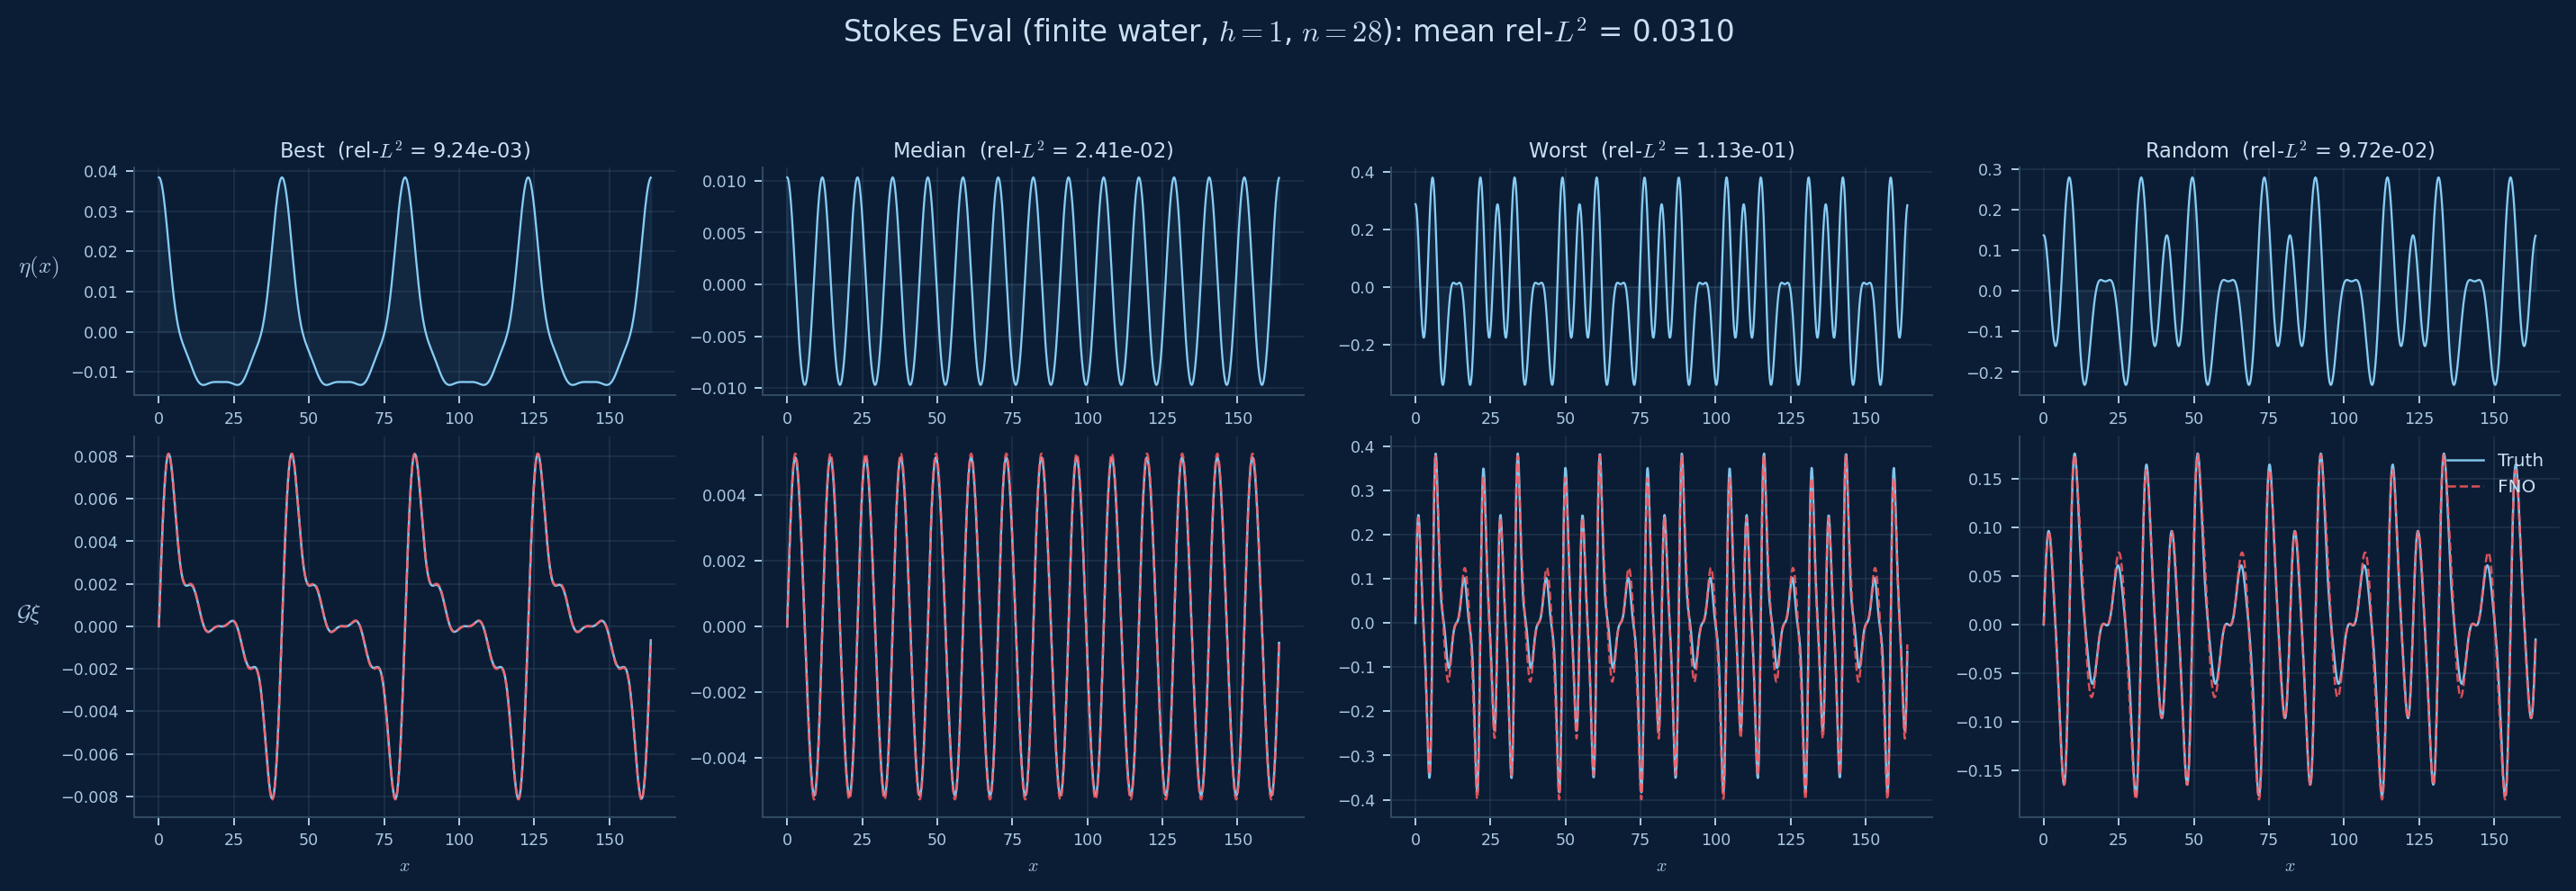
\includegraphics[width=\linewidth,height=0.85\textheight,keepaspectratio]{figures/eval_stokes_finite_samples.png}
\end{frame}

% ============================================================
\begin{frame}{Generalization to Linear Waves ($h = 1$)}

\textbf{Not in training data.} Linear wave superpositions at $h = 1$.

\pause

\begin{center}
\begin{tabular}{lc}
\toprule
Metric & Value \\
\midrule
Mean $\relltwo$   & $\mathbf{0.106}$ \\
Median $\relltwo$ & $0.093$ \\
Std $\relltwo$    & $0.066$ \\
P95 $\relltwo$    & $0.229$ \\
P99 $\relltwo$    & $0.291$ \\
\bottomrule
\end{tabular}
\end{center}

\pause

\textbf{Why so high?} Despite the name ``linear,'' these samples use $\xi$ evaluated on the exact free surface $z = \eta(x)$ via $\cosh(k_0(\eta + h))$, so the DNO has genuine nonlinear content. The issue is \textbf{distribution shift}: these are single-trig-mode cosines at $h = 1$ with steepness up to $k_0 a_0 \approx 2.3$, a profile shape and steepness range absent from training data (solitons + broadband random sea).
\end{frame}

% ============================================================
\begin{frame}{Linear Eval: Samples \& Error Distribution}
\centering
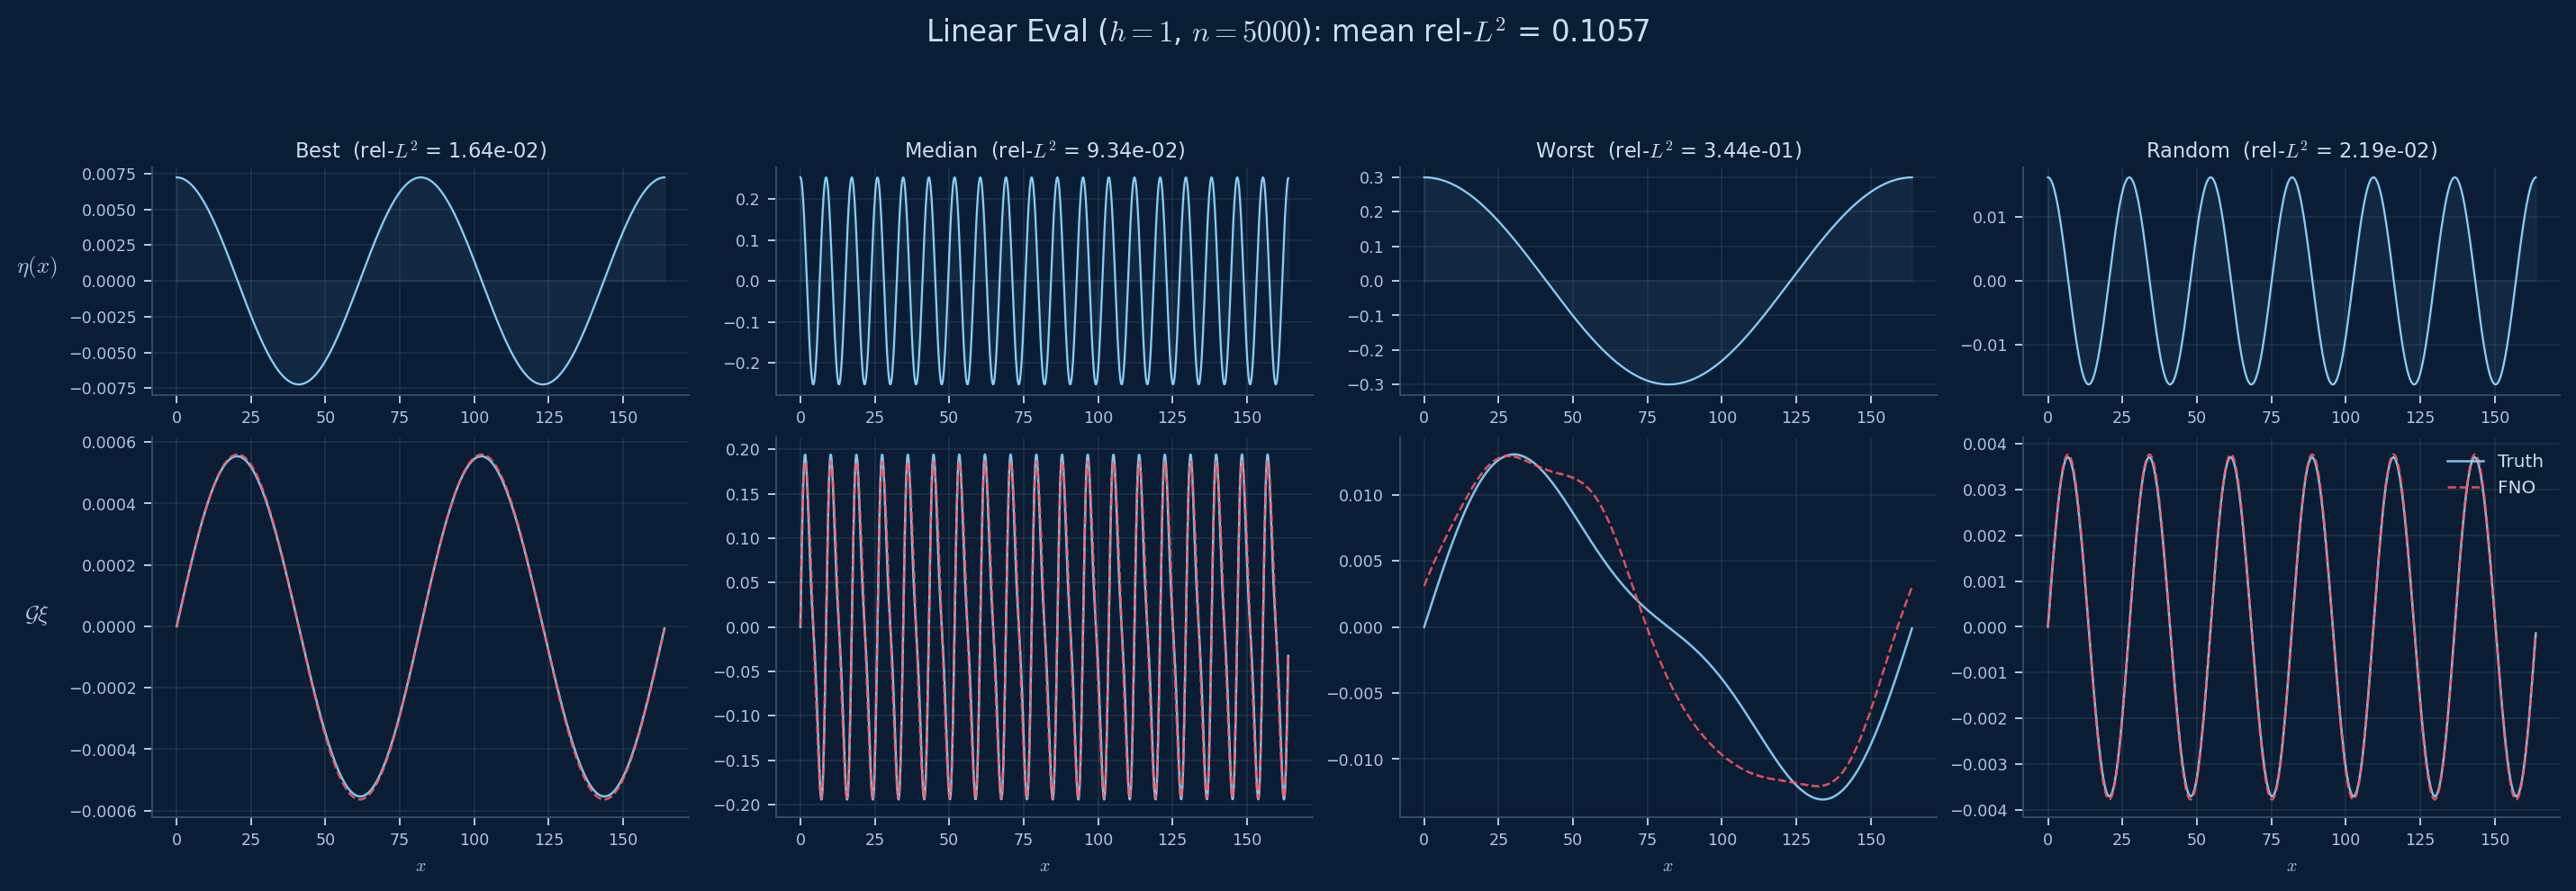
\includegraphics[width=\linewidth,height=0.42\textheight,keepaspectratio]{figures/eval_linear_samples.png}
\vspace{0.2em}
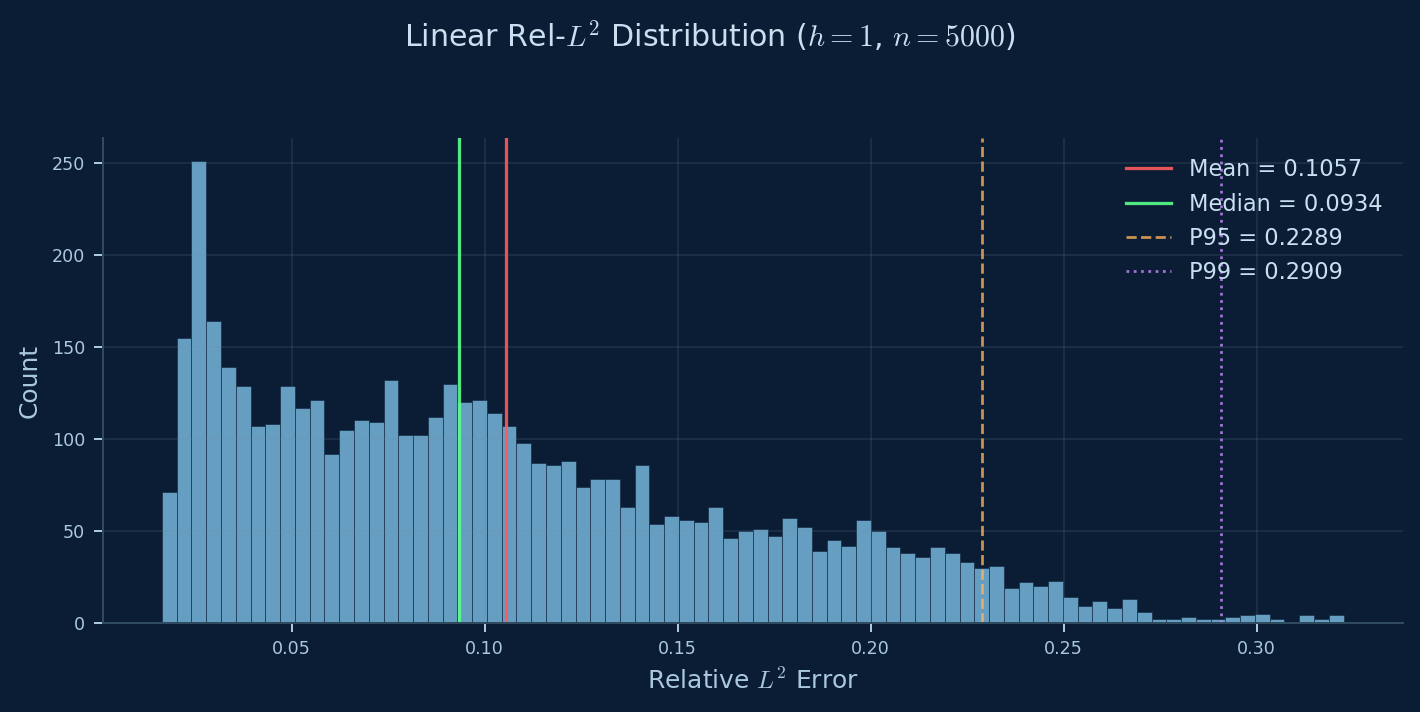
\includegraphics[width=0.75\linewidth,height=0.42\textheight,keepaspectratio]{figures/eval_linear_hist.png}
\end{frame}

% ============================================================
\section{Surrogate Rollouts}

% ============================================================
\begin{frame}{Surrogate Time Integration}

Replace $\Gop(\eta;h)\xi$ with the FNO in the time integrator:
\begin{align*}
  \eta_t &= \hat\Gop_\theta(\eta,\xi;h) - G_0\xi, \\
  \xi_t &= -\tfrac{1}{2}\xi_x^2 + \frac{(\hat\Gop_\theta + \eta_x\xi_x)^2}{2(1+\eta_x^2)}.
\end{align*}

\textbf{Same GL2-IF integrator} as the truth solver. Same substeps (8), same $\tfrac{2}{3}$-rule filter.

\pause

The only change is swapping \texttt{dno\_series\_eval} $\to$ \texttt{FNO.apply}.

\pause

\textbf{Speedup:} The Craig--Sulem series requires $O(M \cdot N \log(8N))$ per evaluation ($M = 6$, $N = 1024$). The FNO forward pass is dominated by 2 spectral blocks with 32-mode convolutions.
\end{frame}

% ============================================================
\begin{frame}{Rollout Accuracy: Short Time ($T = 40$)}

\begin{center}
\begin{tabular}{llcc}
\toprule
Scenario & Depth & $\bar\eta$ mean $\relltwo$ & $\bar\eta$ final $\relltwo$ \\
\midrule
Single soliton ($a = 0.40$)
  & $h = 1$ & 3.1\% & 6.1\% \\
Deep Stokes ($n_0 = 10$, $a_0 = 0.05$)
  & $h = 1000$ & 0.21\% & 0.43\% \\
Finite Stokes ($n_0 = 14$, $a_0 = 0.10$)
  & $h = 1$ & 14.7\% & 24.6\% \\
\bottomrule
\end{tabular}
\end{center}

\pause

The deep-water Stokes rollout is nearly exact ($0.2\%$ mean error over $T = 40$).

The soliton rollout at $3\%$ mean error demonstrates stable propagation of a highly nonlinear wave ($a/h = 0.4$).

Finite-depth Stokes is more challenging due to wave--bottom interaction effects not well-represented in training data.
\end{frame}

% ============================================================
\begin{frame}{Rollout Accuracy: Long Time ($T = 400$--$600$)}

\small{
\begin{center}
\begin{tabular}{lcccc}
\toprule
Scenario & $T_{\max}$ & $\bar\eta$ mean & $\bar\eta$ final & $\bar\xi$ mean \\
\midrule
\multicolumn{5}{l}{\textit{Soliton overtaking collisions ($h = 1$):}} \\
\quad 4:1 amplitude ratio  & 600 & 6.4\% & 20.2\% & 1.7\% \\
\quad 3.5:1 (large amp)    & 600 & 4.1\% & 9.1\%  & 1.7\% \\
\midrule
\multicolumn{5}{l}{\textit{Three-soliton interactions ($h = 1$):}} \\
\quad Equal amps (0.38/0.37/0.26) & 400 & 15.0\% & 42.7\% & 5.5\% \\
\quad Spread amps (0.38/0.35/0.12) & 400 & 7.4\% & 17.0\% & 2.6\% \\
\bottomrule
\end{tabular}
\end{center}
}

The FNO surrogate tracks \textbf{soliton overtaking collisions} through hundreds of time units. Clean overtaking (large amplitude ratio, fast collision) has lower error than slow, prolonged interactions.

Three-soliton dynamics are captured qualitatively, with the spread-amplitude case staying below $7.5\%$ mean error over $T = 400$.
\end{frame}

% ============================================================
\section{Wall-Clock Performance}

% ============================================================
\begin{frame}{Wall-Clock Benchmark (GPU, $N_x = 1024$)}
\small{
\begin{center}
\begin{tabular}{llccc}
\toprule
Operation & Method & Mean (ms) & Min (ms) & Speedup \\
\midrule
\multicolumn{5}{l}{\textit{Single $\Gop$ evaluation (batch = 1):}} \\
& DNO series ($M\!=\!6$, pad $8\times$) & 3.17 & 1.22 & --- \\
& FNO (2 blocks, 32 modes)              & 2.26 & 0.21 & $1.4\times$ \\
\midrule
\multicolumn{5}{l}{\textit{Single $\Gop$ evaluation (batch = 64):}} \\
& DNO series & 3.55 & 2.00 & --- \\
& FNO        & 2.19 & 0.28 & $1.6\times$ \\
\midrule
\multicolumn{5}{l}{\textit{Full GL2-IF time step (1 sample, 4 iterations):}} \\
& DNO series & 21.1 & 17.5 & --- \\
& FNO surrogate & 3.2 & 1.2 & $\mathbf{6.6\times}$ \\
\bottomrule
\end{tabular}
\end{center}


The raw operator speedup is modest ($1.4$--$1.6\times$) since both are FFT-bound at $N = 1024$. But a full GL2-IF step requires $\sim$20 recursive DNO evaluations (order-6 series $\times$ 2 stages $\times$ 4 iterations), yielding \textbf{6.6$\times$} end-to-end speedup per time step.
}
\end{frame}

% ============================================================
\section{Summary}

% ============================================================
\begin{frame}{Summary}

\begin{enumerate}
  \item \textbf{Solver:} Modified Tanaka ICs + GL2-IF time stepper for the Zakharov--Craig--Sulem system
  \item \textbf{Data:} 100k Tanaka solitons ($h = 1$) + 100k random sea ($h = 1000$) = 200k training samples
  \item \textbf{Architecture:} 147k-parameter FNO with linear DNO baseline, FiLM depth conditioning, Sobolev loss
  \item \textbf{Pointwise accuracy:}
    \begin{itemize}
      \item Tanaka solitons: $0.12\%$ mean $\relltwo$
      \item Deep Stokes (OOD): $0.05\%$ mean $\relltwo$
      \item Finite-depth Stokes (OOD): $3.1\%$ mean $\relltwo$
    \end{itemize}
  \item \textbf{Rollout stability:} Surrogate tracks soliton collisions and 3-wave interactions through $T = 400$--$600$ with $4$--$15\%$ mean error
\end{enumerate}
\end{frame}

% ============================================================
\begin{frame}{Next Steps}

\begin{itemize}
  \item Add intermediate depths ($h = 2, 5, 10, 50$) to the training set for smoother depth interpolation
  \item Wall-clock benchmarks: DNO series vs.\ FNO on GPU at various resolutions
\end{itemize}
\end{frame}

\end{document}

